% \documentclass[print, bachelor, vlined]{DissertUESTC}
\documentclass[bachelor, vlined]{DissertUESTC}

\usepackage{svg}
\usepackage{pdfpages}
\usepackage{graphicx}
\usepackage{pgfplots}
\usepackage{bm}

\pgfplotsset{compat=1.18}
\usepgfplotslibrary{statistics}
\usepgfplotslibrary{polar}

\begin{document}

	% 以下两条命令为高亮示例文档中的关键内容而设，正式撰写时切不可使用
	% \newcommand{\shad}[1]{\textcolor{DodgerBlue}{\ttfamily #1}}
	% \newcommand{\shadcmd}[1]{\shad{$\backslash$#1}}


	% 下方命令允许跨页排版包含多个行间公式的公式组，可选参数可取值为1,2,3,4，越大表示跨页倾向越高
	% \allowdisplaybreaks[3]


	% 当论文中某节的内容接近填满页面且其下紧随几项标题时，LaTeX更倾向于在后续的标题前分页，并且纵向拉伸当前页内容的段间距，以实现纵向分散对齐，也就是很多人在问的现象。这并不是模板bug，而是LaTeX特性。
	% 出现这种情况的本质原因是用户的内容，尤其是在页面中有些图、表、标题的时候，它们的高度很可能不是正文行距的整数倍，那必然就会出现这种问题。
	% 如果你觉得Word从上到下直接堆叠内容，然后在页尾留下明显空白的处理方式更合你意，那就使用下方的\raggedbottom命令
	% \raggedbottom  % 此命令可让LaTeX像Word那样直接堆叠页面内容，而不再默认拉伸段间距，代价是页尾可能会有明显空白


	% \setconfidential命令用于设置论文封面中的“密级信息”。慎用！！！学生个人不应随意将论文定性为涉密，需要先经过审批。此命令必须先于\uestccover使用才有效
	% 命令参数：\setconfidential(<信息右上角与纸张左、上边界的距离，以逗号分隔>)[<字体格式>]{<密级>}{<保密期限>}。可选参数默认值：(18cm,2cm)[\zihao{4}\bfseries]
	% \setconfidential{密级}{保密期限}  % 非涉密论文一定要注释掉该命令

	% 封面示例————“双学位学士”以外的学位论文
%	\uestccover[<学院名称排版风格>]{<论文题目>}{<学科专业>}{<学号>}{<作者姓名>}{<指导教师>}{<教师职称>}{<学院>} % 单学位学士、研究生通用

	\uestccover{基于数据插补的电源系统多采样率过程异常检测方法研究}
	{自动化}
	{2022060908009}
	{刘俊}
	{邱根}
	{高级工程师}
	{自动化工程学院}  % 空封面

%	\uestccover{基于数据插补的电源系统多采样率过程异常检测方法研究}
%	{自动化}
%	{2022060908009}
%	{XXX}
%	{XXX}
%	{XXX}
%	{自动化工程学院}  % 空封面

	% 开启中文摘要
	\zhabstract

	随着智能制造的推进，现代工业系统逐渐变得大型化、复杂化，典型工业装置如电源系统集成了大量不同采样率的传感器，统一时间轴后会产生大量结构性缺失值，给异常检测任务带来较大困难。鉴于大功率供能系统在各工业领域发挥着重大作用，及时对其运行状态进行检测、避免发生严重故障具有重要研究意义。逆变器系统是电源系统的关键功率单位，若长期工作在高负载工况下，其内部功率开关、滤波电容、电感等易发生故障，鉴于其状态监测数据多采样率的特点，有必要提出针对性的异常检测方法实现精准监测。然而针对多采样率场景，现有方法大多通过简单插值、降采样或直接忽略缺失值来处理，无法兼顾变量间耦合关系、周期频谱特征与全局时序演化规律。为解决该问题，本文首先构建基于变分自编码器与Transformer的VAE-Former（Variational Auto-Encoder Transformer）验证模型，并进一步提出一种面向多采样率电源系统的自适应图--频率异常检测网络（Adaptive Graph-Frequency Anomaly Detection Network, AGF-ADNet）。

    （1）针对多采样率对齐后结构性缺失破坏时序连续性、现有插补方法局部平滑易受局部误差影响并干扰后续异常判别的问题，设计 VAE-Former 验证模型，通过潜变量建模隐藏状态，以应对多采样率导致的结构性缺失，利用掩码感知变分自编码器完成缺失值补全，再通过采样率感知 Transformer 进行全局重构检测，以验证先插补后检测范式在多采样率异常检测中的可行性。

    （2）针对现有方法难以在结构性缺失条件下联合刻画变量耦合关系、周期频谱特征与全局时序演化规律的问题，提出 AGF-ADNet 模型，在插补阶段，构建双专家协同插补模块，其中自适应图重构专家通过动态图学习与图卷积传播挖掘变量间隐式关联，频域重构专家借助傅里叶变换与频率注意力增强周期性与谐波信息，经采样率感知门控融合模块生成最终插补结果；检测阶段应用采样率感知 Transformer 重构检测器编码采样率信息，联合重构偏差、双专家分歧和分布漂移构建异常评分，实现插补与检测的协同优化。

    在三相全桥逆变系统多采样率测试集上，VAE-Former 取得91.65\%的准确率，证明了显式插补的有效性；AGF-ADNet 进一步取得 99.10\% 的准确率，较本实验中表现最优的对比方法提升12.18\%。实验结果表明，本文方法能够在当前数据条件下缓解多采样率场景中的结构性缺失问题，并提升电源系统异常检测的准确性。

	% 中文关键字
	\zhkeywords{异常检测，多采样率，数据插补，图卷积网络，频域注意力，电源系统}

	% 开启英文摘要
	\enabstract
	With the advancement of intelligent manufacturing, modern industrial systems have gradually become larger and more complex. Typical industrial devices such as power systems integrate a large number of sensors with different sampling rates. After these variables are aligned onto a unified time axis, a large number of structured missing values are generated, bringing considerable difficulties to anomaly detection tasks. Since high-power energy supply systems play an important role in various industrial fields, timely detection of their operating states and prevention of serious faults are of great research significance.

	The inverter system is a key power unit in power systems. If it works under high-load conditions for a long time, its internal power switches, filter capacitors, inductors, and other components are prone to faults. Considering the multi-rate characteristics of its condition monitoring data, it is necessary to propose targeted anomaly detection methods to achieve accurate monitoring. However, for multi-rate scenarios, most existing methods rely on simple interpolation, down-sampling, or direct omission of missing values, and cannot take into account inter-variable coupling relationships, periodic spectral features, and global temporal evolution patterns simultaneously. To solve this problem, this thesis first constructs a VAE-Former (Variational Auto-Encoder Transformer) validation model, and further proposes an Adaptive Graph-Frequency Anomaly Detection Network (AGF-ADNet) for multi-rate power systems.

	(1) To address the problem that structured missing values after multi-rate alignment destroy temporal continuity, while existing imputation methods based on local smoothing are easily affected by local errors and interfere with subsequent anomaly discrimination, a VAE-Former validation model is designed. The model uses latent variables to model hidden states so as to handle the structured missing values caused by multi-rate sampling. It completes missing-value imputation through a mask-aware variational autoencoder, and then performs global reconstruction detection through a rate-aware Transformer, thereby verifying the feasibility of the imputation-before-detection paradigm in multi-rate anomaly detection.

	(2) To address the problem that existing methods have difficulty jointly characterizing inter-variable coupling relationships, periodic spectral features, and global temporal evolution patterns under structured missing conditions, the AGF-ADNet model is proposed. In the imputation stage, a dual-expert collaborative imputation module is constructed. The adaptive graph reconstruction expert mines implicit inter-variable associations through dynamic graph learning and graph convolutional propagation, while the frequency-domain reconstruction expert enhances periodic and harmonic information with the aid of Fourier transform and frequency attention. The final imputation results are generated through a rate-aware gated fusion module. In the detection stage, a rate-aware Transformer reconstruction detector is applied to encode sampling-rate information, and anomaly scores are constructed by combining reconstruction deviation, dual-expert disagreement, and distribution drift, thereby realizing the collaborative optimization of imputation and detection.

	Under the multi-rate test set and evaluation protocol constructed from a three-phase full-bridge inverter experimental platform in this thesis, VAE-Former achieves an accuracy of 91.65\% on the test set, demonstrating the effectiveness of explicit imputation. AGF-ADNet further achieves an accuracy of 99.10\%, improving by 12.18 percentage points over the best-performing comparison method in this experiment. These results indicate that the proposed method can alleviate the structured missing-value problem under the current data conditions and improve the accuracy and robustness of anomaly detection in power systems.

	% 英文关键字
	\enkeywords{Anomaly Detection, Multi-rate Process, Data Imputation, Graph Convolutional Network, Frequency-domain Attention, Power System}


	\tableofcontents  % 主目录，必要

	% \listoffigures  % 图多则放，反之不放

	% \listoftables  % 表多则放，反之不放

	% \listofsymbs  % 生成主要符号表标题，需要额外维护符号表内容

	\chapter{绪论}

	\section{电源系统异常检测研究背景与意义}

    随着工业4.0和智能制造的不断推进，现代工业系统正朝着大型化、复杂化和智能化方向发展\citess{JAVAID2023100001,article,2023MeasS..2800822R}。电源系统、逆变器系统以及典型流程工业装置中集成了大量传感器、执行器与控制单元，系统内部存在电磁、热力、机械和控制等多重耦合关系\citess{article1,LIU2023121075}，运行过程呈现出动态性、非线性和不确定性特征\citess{10.1016/j.eswa.2023.121024}。一旦关键设备退化、控制偏差累积\citess{https://doi.org/10.1049/stg2.70024}或外部工况突变而未被及时识别，就可能引发局部失稳、连锁故障甚至停机事故\citess{KHAN202133,info14100540,article2,Yu_2021}，造成设备损坏、产品质量下降和经济损失。面向复杂工业过程开展可靠的异常检测研究，无论在理论上还是工程上都具有重要意义\citess{tayeh2021anomaly,app11073186}。

    电源系统中的逆变器承担直流电与交流电之间的能量变换任务，是连接电源、负载和控制系统的关键功率单元。以三相全桥逆变器为例，绝缘栅双极型晶体管（Insulated Gate Bipolar Transistor, IGBT）通常作为核心功率开关器件，其兼具较高电压耐受能力、较大载流能力和较快开关速度，因而被广泛用于现代工业、交通运输和电力系统等场景\citess{20241,fei_liu_design_2009}。但在长期高负载、高温、高压、频繁开断以及过流、过压冲击条件下，IGBT 及其外围滤波电感、电容、驱动和连接结构可能出现热失效、电气失效、机械应力失效或封装退化等问题\citess{20241}。这些物理退化会进一步反映到电压、电流、功率、频率、谐波和温度等状态变量中，形成突变、漂移、振荡增强、频谱畸变或波形失真等可观测异常。

    因此，电源系统及其相关工业场景中的异常并非单一统计离群点，而是电磁、热力、机械和控制过程耦合后的综合表现。相比一般静态监测任务，这类系统的异常形态更为多样，单纯依靠人工巡检或固定阈值规则已难以满足实时监测和早期预警的需求。近年来，随着工业现场运行数据的持续积累，数据驱动方法为异常检测提供了新的研究路径。通过挖掘多变量时间序列中的演化规律与变量间的关联结构，即使缺乏完备的机理模型，也能够在一定程度上识别设备健康状态和过程异常。

    然而，真实工业数据通常并非理想的单采样率序列。大型系统中往往部署了多类型传感器网络，可以同时采集量纲不同、数值差异较大的各类状态参量。由于传感器成本、测量原理、通信带宽和变量动态特性存在差异，不同变量通常以不同频率采集。例如，电流、电压等电气量一般以较高频率采样，而温度、状态量或质量指标则以较低频率更新。将这些不同采样率的数据统一对齐到同一时间轴后，会产生大量规则性缺失值和时间异步现象，形成多采样率时间序列。这种特性一方面削弱了数据完整性，另一方面增加了建模难度——直接套用单采样率异常检测方法难以充分利用低频变量信息，还可能因缺失值传播、插补失真和时序错位而降低检测精度。

    基于上述背景，围绕多采样率工业过程数据开展异常检测研究，尤其是探索数据插补与异常检测协同优化的建模思路，兼具理论和工程两方面意义。在理论上，相关研究有助于深化对多采样率时间序列表示、缺失信息恢复以及异常模式判别机制的认识，丰富工业过程监测与智能诊断的方法体系。在工程上，通过软件建模手段提升对低频变量和隐性异常的感知能力，可以在一定程度上降低对高成本高频传感器的依赖，为电源系统及相关工业场景的安全运行、故障预警和运维决策提供支撑。

	\section{单采样率异常检测方法研究现状}

	\subsection{基于统计与机器学习的单采样率异常检测研究现状}

    异常检测的早期研究主要基于统计学建模、距离与密度度量、聚类分析以及支持向量机等方法。统计学方法通过假设数据服从特定分布\citess{2010EnvMS..25.1014H}并设置判别阈值来识别异常\citess{doi:10.1137/S0036144500371907}，实现简单且计算开销较低；基于距离、密度和聚类的方法利用样本间相似性关系识别离群行为\citess{e71595caf5ab496585138be92401f5e8,KUMPULAINEN20083840,10.1145/331499.331504,2007ITKDE..19..345G,Muniyandi2012NetworkAD}；单类支持向量机等判别式方法在缺乏异常样本时也有一定适用性\citess{HIMEUR2021116601}。这些方法在结构较简单、维度较低且分布相对稳定的场景中取得了较好的效果。

    但面对复杂工业过程，传统方法的局限性较为明显。多数方法依赖显式分布假设或人工设计特征\citess{Davis2011DataPF}，当系统呈现强非线性、强耦合和时变特性时，模型鲁棒性往往不足。此外，在高维多变量场景下，距离和密度度量的判别能力会受到维度影响，聚类效果对参数和特征选择也比较敏感\citess{SURESH2024112369,DU2024121161}。传统方法还难以刻画长时间跨度内的动态依赖关系，对复杂异常模式和多类型故障的适应能力有限\citess{Rezaei2021ANS}。随着工业数据规模和复杂度不断提升，仅依靠传统方法已难以满足高精度和实时异常检测的需求。

	\subsection{基于深度学习的单采样率异常检测研究现状}

    深度学习方法能够通过端到端训练自动提取时序特征，在高维、非线性和强噪声场景中具有较强的建模能力，已成为异常检测领域的重要研究方向。现有研究大体分为两类：一类是基于预测的方法，利用历史序列预测未来观测值，将预测误差作为异常判据；另一类是基于重构的方法，通过自编码器、变分自编码器或 Transformer 等模型学习正常样本的潜在表示，再根据重构误差识别异常。

    以长短期记忆网络（Long Short-Term Memory, LSTM）、时序卷积网络（Temporal Convolutional Networks, TCN）和 Transformer 为代表的深度时序模型在工业异常检测中得到了广泛应用。LSTM 擅长建模时间依赖关系，TCN 具有并行效率高和感受野可扩展的特点，Transformer 则依靠自注意力机制在长序列建模方面表现突出。与传统方法相比，深度学习模型减轻了对人工特征工程的依赖，适合处理复杂工业系统中的高维动态数据。

    尽管如此，现有深度学习异常检测方法仍存在不足。多数方法默认所有变量具有统一采样率\citess{hu2021lstm}，对多采样率场景下的规则性缺失和时间异步问题考虑不足；很多模型主要聚焦时间维度建模，对变量间耦合关系和频域信息的利用仍不充分；此外，异常阈值的设定、噪声干扰的抑制以及模型可解释性等问题在实际部署中也仍然突出。

	\section{多采样率异常检测研究现状}

    受限于传感器部署成本、测量技术条件以及物理变量本身的动态特性差异，工业过程所采集的数据普遍呈现出多采样率的显著特征\citess{Wen2025AMF,proceedings2130781,2024PatRe.14509943C}，其核心特征在于数据中包含大量因采样频率差异而产生的缺失值\citess{YANG2023109410}。随着智能制造和工业物联网（Industrial Internet of Things, IIoT）的发展，越来越多的设备配备了不同类型的传感器，用于采集实时运行状态和性能数据。这些传感器的差异不仅体现在硬件类型上，也反映在各自的采样频率上，由此导致统一对齐后的数据集——尤其是低频采样变量——不可避免地包含大量缺失值。这些缺失值直接影响数据的完整性和一致性，使得后续分析和建模工作更加复杂\citess{YUAN202011883}。在故障检测任务中，缺失值可能掩盖潜在的故障信号或干扰模型的学习过程，降低检测的准确性和可靠性。同时，不同变量之间既存在时序相关性，又存在空间与功能层面的耦合关系，给多采样率数据的建模带来了较大挑战。如何在多采样率环境下合理处理缺失值，是当前故障检测算法研究中的一个重要问题。现有方法大致可归纳为三类：降采样法、直接建模方法和数据插补方法。

    \subsection{基于降采样的多采样率异常检测研究现状}

    降采样方法将数据按照统一的采样频率重新排列，通过丢弃部分数据将高频采样变量降至与低频采样变量相同的采样率。

    这类方法往往无法适应多采样率环境下的数据特点，可能导致高频变量中的重要动态信息丢失，降低模型对快速变化过程的感知能力，同时引入人为噪声，破坏数据原有的时间依赖结构\citess{Huang2025AttentionBasedMN}。Lu 等人（2024）指出，将多采样率多变量时间序列（Multirate Multivariate Time Series, MR-MTS）强制转换为统一采样率的序列，容易导致信息丢失或结构失真\citess{liu_multirate-former_2024,lu_unmanned_2024}。因此，研究者正在探索能够兼顾缺失值填补与采样频率差异的处理方案，以更充分地利用多采样率数据提升故障检测性能。

    \subsection{基于直接建模的多采样率异常检测研究现状}

    另一类研究致力于设计端到端模型，直接对多采样率数据进行建模，以避免显式插补带来的误差积累。Lu 等人（2024）提出的多采样率感知长短期记忆网络（Multirate-Aware LSTM, MRA-LSTM）是该方向的代表性工作\citess{lu_unmanned_2024}。

    早期研究中，LSTM Units Achieves（LSTMa）\citess{Bahdanau2014NeuralMT}和LSTM Time-Series Network（LSTNet）\citess{10.1007/s11063-022-10950-2}等模型通过将时间依赖关系划分为长期影响与短期依赖，并引入注意力机制来提取多尺度特征，在一定程度上缓解了缺失值带来的影响。然而，当多采样率问题较为严重时，这类模型依赖的参数共享策略可能难以有效刻画不同采样频率变量的异质演化规律。Lu 等人（2024）提出的MRA-LSTM通过引入多采样率感知结构和多尺度更新机制，能够在时间维度上权衡不同频率信息的重要性，避免高频变量对低频变量依赖关系的掩盖。其核心思想在于：如果模型能够明确“感知”每个输入样本的采样率或时间间隔，并在推理过程中加以区分，则无需对数据进行强制对齐，也能学习到真实的时序依赖关系。已知大多数推理过程在每个时间步执行，高采样率数据获得更多参与推理的机会。为了避免这一情况，该网络以多个传感器时间序列作为输入，统一构建时间轴，对低频数据使用最近邻/保持，对高频数据保留原始时间步，并提出采样率感知编码

    MRA-LSTM 的研究表明了多尺度特征融合的重要性，对后续设计基于插补的异常检测模型具有参考价值。但该方法在处理缺失值时存在不足：其策略是直接忽略缺失值，未对缺失数据进行合理的补全。这种处理方式可能导致数据中的潜在模式和关键信息被丢弃，限制了模型对样本演变规律的学习效果。

    Song 等人提出了多时序通道卷积神经网络（Multitemporal Channels Convolutional Neural Network, MC-CNN）\citess{song_soft_2025}，利用改进的反向传播（Back Propagation, BP）算法处理带有缺失值的输入序列，然后通过卷积神经网络进行局部特征提取，再经全连接层映射。MC-CNN 在局部特征提取方面取得了一定成果，但与 MRA-LSTM 类似，其对缺失值仍采用简单的忽略策略，可能导致潜在关键信息的丢失，影响预测精度和泛化能力。Zhou 等人提出了多采样率因子分析模型（MR-FA）\citess{zhou_multirate_2019}。MR-FA 假设所有不同采样率的测量值都共享同一组公共潜在因子 $t(k)$，通过这些因子来界定和约束变量间的互相关性，其核心仍基于静态因子分析，对于具有显著动态时域特性的工业过程（如具有时滞或动态演化特征的系统），其捕捉变量间时序动态信息的能力尚存在提升空间。

    综合来看，尽管已有多采样率直接建模方法在一定程度上缓解了采样频率差异带来的问题，但在数据缺失和信息不完整的场景下仍面临挑战。简单的忽略策略难以利用缺失位置所蕴含的时序关联信息，缺失值若不经合理的插补处理，可能导致潜在模式丢失，影响模型的故障检测能力。

    \subsection{基于数据插补的多采样率异常检测研究现状}

    基于数据插补的方法首先将所有变量按照最高采样率在时间轴上对齐，然后通过建模方法填补缺失点以得到完整数据集，最后在此基础上进行异常检测。

    Liu 等人提出了一种基于 Transformer 的多层多采样率网络（Multirate-Former）\citess{liu_multirate-former_2024}，该方法引入采样率编码，先通过多层卷积神经网络学习局部特征并进行粗粒度数据补全，随后将采样率和相位信息嵌入位置编码中，利用 Transformer 进行异常检测。但该方法对数据全局信息的利用不够充分，整体检测效果有限。

    Xin 等人提出了一种面向工业控制与物联网系统（Industrial Cyber-Physical Systems, ICPSs）的多采样率异常检测方法\citess{10494703}，采用机制模型（Mechanism Model, MM）在时间域和空间域对数据进行超分辨率处理以填补缺失数据，并通过扩展虚拟空间状态来补充数据特征。然而，机制模型依赖于对特定系统物理特性和工程特性的先验知识，建模难度较高且自适应性较差。

    总体而言，数据插补方法在一定程度上解决了不同采样率数据在异常检测中作用不平衡的问题，使得低频变量信息得以利用，降低了建模难度，但现有方法的插补精度和适应性仍有待提升。

    \section{相关理论与关键技术}

    多采样率工业过程异常检测涉及变量关系建模、频域结构分析以及长程依赖建模等多个方面。为此，本文在模型设计中综合引入图卷积网络、时序卷积网络、傅里叶变换与 Transformer 等关键技术。本章围绕上述三类方法展开介绍，重点说明其基本思想、核心公式、主要特点及其在工业时间序列建模中的适用性，为后续章节的方法设计与实验分析提供理论基础。

    \subsection{图卷积网络}

    \subsubsection{图结构表示}

    与规则网格数据不同，工业系统中的多变量关系通常具有显著的非欧式结构特征。例如，电压、电流、功率、温度和状态量之间往往存在复杂的物理耦合与控制耦合，这类关系难以用传统的一维或二维卷积直接表示。图结构能够以更加自然的方式描述变量之间的关联，因此适合用于工业多变量数据建模。

    一般将图表示为
    \begin{equation}
        \mathcal{G} = (\mathcal{V}, \mathcal{E}, \mathbf{A}),
    \end{equation}
    其中，$\mathcal{V}$ 表示节点集合，$\mathcal{E}$ 表示边集合，$\mathbf{A} \in \mathbb{R}^{N \times N}$ 表示邻接矩阵，$N$ 为节点数。当节点 $i$ 与节点 $j$ 存在连接关系时，$A_{ij} > 0$；否则 $A_{ij} = 0$。若每个节点都带有特征向量，则可定义节点特征矩阵
    \begin{equation}
        \mathbf{X} = [\mathbf{x}_1, \mathbf{x}_2, \ldots, \mathbf{x}_N]^\top \in \mathbb{R}^{N \times F},
    \end{equation}
    其中 $F$ 为节点特征维数。

    在工业过程场景中，可以将每个传感器变量视为一个节点，将变量间的统计相关性、物理耦合关系或数据驱动学习得到的依赖关系视为边。这样，复杂多变量系统就被转化为图上的特征传播与表示学习问题。

    \subsubsection{图卷积的基本原理}

    图卷积网络（Graph Convolutional Network, GCN）的核心思想是通过节点与其邻居之间的消息传递，实现图结构上的局部特征聚合。对于节点 $i$ 而言，其更新后的表示不仅依赖于自身特征，也依赖于邻居节点的信息。因此，图卷积可以看作一种基于拓扑结构的加权邻域平均。

    经典 GCN 的一层传播公式可写为
    \begin{equation}
        \mathbf{H}^{(l+1)} =
        \sigma\!\left(
            \hat{\mathbf{D}}^{-1/2}
            \hat{\mathbf{A}}
            \hat{\mathbf{D}}^{-1/2}
            \mathbf{H}^{(l)}
            \mathbf{W}^{(l)}
        \right),
    \end{equation}
    其中，$\mathbf{H}^{(l)}$ 表示第 $l$ 层输入特征，$\mathbf{W}^{(l)}$ 为可学习权重矩阵，$\sigma(\cdot)$ 为非线性激活函数，$\hat{\mathbf{A}} = \mathbf{A} + \mathbf{I}$ 表示加入自环后的邻接矩阵，$\hat{\mathbf{D}}$ 为对应的度矩阵，即
    \begin{equation}
        \hat{D}_{ii} = \sum_j \hat{A}_{ij}.
    \end{equation}

    上述公式包含三个关键步骤。首先，通过加入单位矩阵 $\mathbf{I}$ 为每个节点保留自环，使节点在聚合邻居信息时不会丢失自身表示。其次，通过 $\hat{\mathbf{D}}^{-1/2}\hat{\mathbf{A}}\hat{\mathbf{D}}^{-1/2}$ 对邻接矩阵进行对称归一化，避免高度节点在传播过程中产生过强影响，并提升训练稳定性。最后，通过线性变换和非线性映射实现特征空间上的投影与更新。

    \subsubsection{图卷积在本文中的作用}

    本文所研究的多采样率异常检测任务中，不同变量之间存在复杂而隐式的关联关系，仅依靠逐变量时序建模难以充分利用这些信息。图卷积能够在变量维度上实现信息传播，为低频变量的插补和异常状态的识别提供结构约束。因此，图卷积是本文完成跨变量依赖建模的重要基础。

    \subsection{傅里叶变换与频域分析}

    \subsubsection{离散傅里叶变换}

    时间序列既可以在时域中表示，也可以在频域中表示。时域描述信号随时间的变化过程，频域则刻画信号由哪些频率成分组成。傅里叶变换正是完成时域与频域转换的核心工具。

    对于长度为 $N$ 的离散时间序列 $\{x[n]\}_{n=0}^{N-1}$，其离散傅里叶变换（Discrete Fourier Transform, DFT）定义为
    \begin{equation}
        X[k] = \sum_{n=0}^{N-1} x[n] e^{-j 2\pi kn / N}, \qquad k = 0,1,\ldots,N-1,
    \end{equation}
    其中 $j = \sqrt{-1}$ 为虚数单位。对应的逆变换为
    \begin{equation}
        x[n] = \frac{1}{N}\sum_{k=0}^{N-1} X[k] e^{j 2\pi kn / N}.
    \end{equation}

    频谱 $X[k]$ 是复数形式，可以进一步分解为实部、虚部、幅值和相位。其中，幅值 $|X[k]|$ 反映第 $k$ 个频率分量的能量大小，相位 $\angle X[k]$ 则表示其相位偏移。对于工业信号而言，周期振荡、谐波成分和噪声干扰往往在频域中具有更加直观的表现形式。

    \subsubsection{快速傅里叶变换}

    直接计算 DFT 的时间复杂度为 $O(N^2)$，当序列长度较大时计算开销较高。快速傅里叶变换（Fast Fourier Transform, FFT）通过利用复指数项的对称性与周期性，将复杂度降为
    \begin{equation}
        O(N \log N),
    \end{equation}
    从而显著提高了频域分析效率。对于实值序列，还可以采用仅保留非冗余频谱部分的实数快速傅里叶变换（rFFT），进一步降低存储与计算成本。

    因此，FFT 已成为信号处理和深度学习时序建模中最常用的频域分析工具之一。它不仅适用于传统谱分析，也能够与神经网络结合，用于学习频率重要性、增强关键频段表示或构造频域损失函数。

    \subsubsection{频域分析在本文中的作用}

    很多工业异常在时域中的表现并不十分显著，但在频域中往往具有更好的可分性。例如，谐波畸变会导致特定频段能量增强，机械振动异常会表现为主频漂移或边频出现，噪声污染则常表现为高频能量异常增加。因此，引入频域分析有助于从另一种视角揭示异常特征。

    对于多采样率工业数据而言，频域分析还具有两点额外意义。其一，频域表征有助于增强对周期结构和重复模式的建模能力；其二，频域约束可以作为时域重构的补充，缓解单纯依赖均方误差时容易出现的过度平滑问题。当然，在处理缺失值较多或零填充较强的序列时，频域分析也可能受到频谱泄露影响，因此通常需要结合掩码机制、插补策略或频域注意力方法共同使用。

    本文所研究的电源系统及相关工业场景具有明显的周期性与频谱结构特征，部分异常在频域中的可分性优于时域。因而，傅里叶变换为本文构建频域分支、强化谐波与周期特征表达提供了必要基础，是实现时频协同异常检测的重要理论支撑。

    \subsection{Transformer}

    Transformer 是近年来序列建模领域最具代表性的深度学习结构之一，其核心是自注意力机制（Self-Attention）。与卷积和循环结构不同，自注意力能够直接建立序列任意两个位置之间的联系，从而更高效地捕获长距离依赖关系。其结构如图\ref{fig:transformer_structure}所示。

     \begin{figure}[!htbp]
        \centering
        \includegraphics[width=0.9\linewidth]{transformer.drawio.pdf}
        \caption{Transformer结构示意}
        \label{fig:transformer_structure}
    \end{figure}

    \subsubsection{自注意力机制}

    设输入序列表示为
    \begin{equation}
        \mathbf{H} \in \mathbb{R}^{T \times d},
    \end{equation}
    其中 $T$ 为序列长度，$d$ 为特征维数。首先通过线性变换得到查询矩阵、键矩阵和值矩阵：
    \begin{equation}
        \mathbf{Q} = \mathbf{H}\mathbf{W}_Q,\qquad
        \mathbf{K} = \mathbf{H}\mathbf{W}_K,\qquad
        \mathbf{V} = \mathbf{H}\mathbf{W}_V.
    \end{equation}
    然后，自注意力输出为
    \begin{equation}
        \operatorname{Attention}(\mathbf{Q}, \mathbf{K}, \mathbf{V}) =
        \operatorname{softmax}\!\left(
            \frac{\mathbf{Q}\mathbf{K}^{\top}}{\sqrt{d_k}}
        \right)\mathbf{V},
    \end{equation}
    其中 $d_k$ 为键向量维度。上述公式表明，模型会根据查询向量与键向量的相似度，为不同位置分配不同权重，再对值向量进行加权求和。

    \subsubsection{多头注意力与位置编码}

    为了增强模型从不同子空间提取依赖关系的能力，Transformer 通常采用多头注意力（Multi-Head Attention）机制。若共有 $h$ 个注意力头，则第 $i$ 个头的输出为
    \begin{equation}
        \mathrm{head}_i =
        \operatorname{Attention}(\mathbf{Q}_i, \mathbf{K}_i, \mathbf{V}_i),
        \qquad i=1,2,\ldots,h.
    \end{equation}
    将所有头拼接后，再经线性变换得到最终结果：
    \begin{equation}
        \operatorname{MHA}(\mathbf{H}) =
        \operatorname{Concat}(\mathrm{head}_1,\ldots,\mathrm{head}_h)\mathbf{W}_O.
    \end{equation}

    由于自注意力本身对输入顺序不敏感，Transformer 还需要引入位置编码（Positional Encoding）来提供序列位置信息。位置编码可以采用固定的正弦余弦形式，也可以采用可学习参数形式，其本质都是让模型区分不同时间步的相对或绝对位置。

    \subsubsection{前馈网络与编码器结构}

    在标准 Transformer 编码器中，多头注意力模块后通常接有逐位置前馈网络（Feed-Forward Network, FFN），并配合残差连接与层归一化共同构成编码层。设输入为 $\mathbf{Z}_{l-1}$，则第 $l$ 层编码器可表示为
    \begin{align}
        \mathbf{Z}_l' &= \operatorname{LayerNorm}\!\left(
            \mathbf{Z}_{l-1} + \operatorname{MHA}(\mathbf{Z}_{l-1})
        \right), \\
        \mathbf{Z}_l &= \operatorname{LayerNorm}\!\left(
            \mathbf{Z}_l' + \operatorname{FFN}(\mathbf{Z}_l')
        \right).
    \end{align}

    前馈网络一般包含两层线性变换与非线性激活，其作用是对每个时间位置进行更充分的特征映射。残差连接能够改善梯度传播，层归一化则有助于稳定训练过程。通过多层编码器堆叠，Transformer 可以在全局范围内学习复杂的时间依赖与模式交互。

    \subsubsection{Transformer 的作用}

    Transformer 在时间序列建模中的主要优势体现在以下几个方面：

    \begin{itemize}
        \item \textbf{全局依赖建模能力强。} 任意两个时间位置都可以直接建立联系，适合处理长序列依赖关系。
        \item \textbf{表达能力丰富。} 多头机制能够从不同子空间学习多种相关模式，提高特征表示能力。
        \item \textbf{适合与其他模块协同工作。} Transformer 可作为全局建模器，与卷积、图神经网络或频域模块结合，形成混合式时序建模框架。
    \end{itemize}

    本文将 Transformer 作为全局重构模块使用，目的是在完成局部时序特征提取和频域增强后，进一步建模整个时间窗口范围内的长程依赖关系。与图卷积和 TCN 相比，Transformer 更擅长捕捉跨越较长时间跨度的整体演化规律，因此能够为异常评分提供更高质量的重构结果。

	\section{本文研究定位}
	基于现有研究基础，本文围绕电源系统多采样率异常检测问题，针对插补不可靠、变量耦合建模不足及周期性异常感知能力弱等核心问题，首先设计 VAE-Former 验证传统方法的插补和检测能力，用掩码感知 VAE 完成缺失值补全，再利用采样率感知 Transformer 进行全局重构检测。在此基础上，进一步提出融合自适应图结构与频域注意力机制的端到端异常检测模型 AGF-ADNet，通过图学习、频域特征增强和门控融合提升模型对变量耦合关系、周期频谱信息和全局时序演化规律的表达能力。
    \section{论文结构安排}
    除本章外，全文其余部分拟安排如下：
    \begin{itemize}
        \item 第二章介绍两类方法共享的多采样率数据表示、样本构造、采样率感知重构检测器和判别流程，并在此基础上阐述 VAE-Former 验证模型。
        \item 第三章详细阐述 AGF-ADNet 模型，包括自适应图结构学习、时频双分支插补、采样率感知门控融合以及多源异常评分方法。
        \item 第四章利用三相全桥逆变系统实验平台进行验证，给出实验设计、评价指标与对比方法，并对模型在典型多采样率工业过程数据上的检测结果进行分析，验证所提方法的有效性。
        \item 第五章对全文工作进行总结，归纳研究结论，并结合当前方法的局限性展望后续改进方向。
    \end{itemize}

    \chapter{基于VAE-Former的多采样率异常检测方法研究}

    本章面向多采样率电源系统异常检测任务，首先给出两类方法共享的问题定义、数据处理流程和异常判别框架，再在此基础上构建 VAE-Former 验证模型。该章的重点不在于追求最终最优性能，而是验证基于数据结构进行缺失插补--全局重构--异常评分这一基本路线在多采样率数据条件下是否可行，为后续 AGF-ADNet 的结构增强提供依据。

    \section{问题定义}

    面向电源系统多采样率异常检测任务，设原始监测序列记为
    \begin{equation}
        \mathbf{D} = [\mathbf{d}_1,\mathbf{d}_2,\ldots,\mathbf{d}_T]^\top \in \mathbb{R}^{T \times N},
    \end{equation}
    其中，$T$ 表示时间长度，$N$ 表示监测变量数，$\mathbf{d}_t \in \mathbb{R}^{N}$ 表示时刻 $t$ 的多变量观测向量。针对多采样率场景中普遍存在的结构性缺失，引入缺失掩码
    \begin{equation}
        M_{t,n} =
        \begin{cases}
            1, & \text{第 $t$ 个时刻第 $n$ 个变量缺失},\\
            0, & \text{第 $t$ 个时刻第 $n$ 个变量可观测},
        \end{cases}
    \end{equation}
    并定义观测掩码为
    \begin{equation}
        O_{t,n} = 1 - M_{t,n}.
    \end{equation}

    本文采用长度为 $L$ 的滑动窗口构造样本，窗口张量表示为
    \begin{equation}
        \mathbf{X} \in \mathbb{R}^{B \times L \times N}, \qquad
        \mathbf{M} \in \{0,1\}^{B \times L \times N},
    \end{equation}
    其中 $B$ 为批大小。在当前实验设置中，窗口长度取 $L=50$，变量总数为 $N=18$。根据各变量观测频率差异，可进一步将变量划分为若干采样率组，并为每个变量赋予采样率类别标识 $r_n$ 与采样步长 $s_n$。

    VAE-Former 与 AGF-ADNet 均采用先进行缺失插补，再全局重构，最后异常判别的基本范式。设训练或推理阶段模型实际看到的缺失掩码为 $\widetilde{\mathbf{M}}$，则两类方法的共享流程可概括为
    \begin{align}
        \mathbf{X}^{\mathrm{in}} &= \mathbf{X} \odot (1-\widetilde{\mathbf{M}}), \\
        \mathbf{X}^{\mathrm{imp}} &= \mathcal{I}_{\theta}\!\left(\mathbf{X}^{\mathrm{in}},\widetilde{\mathbf{M}},\mathbf{r},\mathbf{s}\right), \\
        \mathbf{X}^{\mathrm{comp}} &= \mathbf{X}^{\mathrm{in}} + \widetilde{\mathbf{M}} \odot \mathbf{X}^{\mathrm{imp}}, \\
        \hat{\mathbf{X}} &= \mathcal{D}_{\phi}\!\left(\mathbf{X}^{\mathrm{comp}},\mathbf{O},\mathbf{r},\mathbf{s}\right).
    \end{align}
    其中，$\mathcal{I}_{\theta}(\cdot)$ 表示插补器，$\mathbf{X}^{\mathrm{comp}}$ 表示由观测值与插补值共同构成的完整窗口，$\mathcal{D}_{\phi}(\cdot)$ 表示采样率感知 Transformer 重构检测器。VAE-Former 使用掩码感知 VAE 作为插补器，用于验证该范式的基本可行性；AGF-ADNet 则将插补器替换为图结构专家与频域专家的门控融合模块，以提升对变量耦合和周期特征的表达能力。

    需要说明的是，本文最终输出正常与异常两类判别结果，但方法设定并非依赖正常样本和故障样本共同训练的普通监督二分类。训练阶段主要利用正常工况样本学习系统在健康状态下的重构规律，并依据训练或验证样本的异常分数分布确定检测阈值；测试阶段再根据样本相对正常模式的偏离程度给出异常分数和二值告警。测试集标签仅用于计算评价指标，不参与模型参数学习。因此，本文所述主要是评价层面的正常/异常判别形式，本质上仍属于基于正常数据建模的异常检测任务。

    \section{数据处理与样本构造}

    \subsection{缺失掩码生成与观测值标准化}

    多采样率工业数据在统一时间轴对齐后，不同变量会在非采样时刻形成大量空缺项。本文以缺失掩码 $\mathbf{M}$ 显式记录该信息，并仅基于可观测位置估计标准化参数。对于第 $n$ 个变量，其均值与标准差定义为
    \begin{align}
        \mu_n &= \frac{\sum_{t=1}^{T} O_{t,n} D_{t,n}}{\sum_{t=1}^{T} O_{t,n} + \varepsilon}, \\
        \sigma_n &= \sqrt{\frac{\sum_{t=1}^{T} O_{t,n}(D_{t,n}-\mu_n)^2}{\sum_{t=1}^{T} O_{t,n} + \varepsilon} + \varepsilon},
    \end{align}
    其中 $\varepsilon$ 为防止分母为零的极小常数。随后，将缺失位置临时以变量均值替代，得到
    \begin{equation}
        \bar{D}_{t,n} = O_{t,n} D_{t,n} + M_{t,n} \mu_n,
    \end{equation}
    并执行标准化变换
    \begin{equation}
        \tilde{D}_{t,n} = \frac{\bar{D}_{t,n}-\mu_n}{\sigma_n}.
    \end{equation}

    这一处理方式具有两点优势：其一，标准化参数仅由真实观测值确定，避免缺失模式对统计量造成偏移；其二，缺失位置在标准化后变为零，从而可与显式掩码协同输入网络。这样既保证不同变量在输入端具有统一的数值尺度，也避免缺失占位值对后续插补器和检测器造成额外干扰。

    \subsection{滑动窗口构造}

    为兼顾局部动态建模与序列级异常评分，本文采用两类窗口化策略。

    \begin{enumerate}
        \item 对于插补训练与全序列补全过程，采用前端填充滑动窗口。若某一时刻历史长度不足 $L$，则以前序首样本进行补齐，使每一个时间索引都对应一个长度为 $L$ 的输入窗口。
        \item 对于异常评分阶段，采用标准滑动窗口，即仅在历史长度达到 $L$ 后开始取窗，以避免前端填充对统计分数带来额外偏差。
    \end{enumerate}

    以前端填充窗口为例，第 $t$ 个时间点对应的窗口样本可表示为
    \begin{equation}
        \mathbf{X}^{(t)} =
        \begin{cases}
            [\underbrace{\tilde{\mathbf{d}}_1,\ldots,\tilde{\mathbf{d}}_1}_{L-t},\tilde{\mathbf{d}}_1,\ldots,\tilde{\mathbf{d}}_{t}], & 1 \leq t < L, \\
            [\tilde{\mathbf{d}}_{t-L+1},\ldots,\tilde{\mathbf{d}}_{t}], & L \leq t \leq T.
        \end{cases}
    \end{equation}

    通过这种方式构建并输入模型的一个窗口如图\ref{fig:windowing}所示。

    \begin{figure}[!htbp]
        \centering
        \includegraphics[width=0.4\linewidth]{窗口.pdf}
        \caption{时间窗口}
        \label{fig:windowing}
    \end{figure}

    相应掩码窗口按完全相同的方式构造。前端填充窗口主要服务于补全输出与原序列的逐点对齐，标准窗口则主要服务于异常评分阶段。二者分别面向补全过程与判别过程的不同需求，有助于兼顾时间对齐精度和评价稳定性。

    \subsection{采样率模式推断与分块}

    对于多采样率过程，变量的观测比例本身包含采样步长信息。设第 $n$ 个变量的观测比例为
    \begin{equation}
        \rho_n = \frac{1}{T}\sum_{t=1}^{T} O_{t,n},
    \end{equation}
    则其采样步长可近似写为
    \begin{equation}
        s_n = \operatorname{round}\!\left(\frac{1}{\max(\rho_n,\varepsilon)}\right).
    \end{equation}
    根据不同步长的取值，可进一步映射为离散采样率类别标识 $r_n$。该元数据在 VAE-Former 与 AGF-ADNet 的 Transformer 编码中共同发挥作用；在 AGF-ADNet 中，还进一步用于门控融合模块。

    同时，基于上述推断得到的采样率组，可以对数据进行分块（chunking）。    
    \begin{figure}[!htbp]
        \centering
        \includegraphics[width=\linewidth]{chunking.drawio.pdf}
        \caption{数据分块示意图}
        \label{fig:data_chunking}
    \end{figure}

    该步骤将相似采样率组的数据排列在一起，相似采样率的变量通常具有较强的相关性，可以使模型更稳定地利用同采样层级变量之间的相关信息。数据分块示意如图\ref{fig:data_chunking}所示。其中红色代表缺失样本。

    \subsection{自监督再遮挡机制}

    原始结构性缺失位置不具备真实标签，因此插补训练不能直接以其作为监督目标。为此，本文在训练阶段从原本可观测的位置中随机抽取一部分进行再遮挡，记为 $\mathbf{R}$。于是模型实际看到的缺失掩码为
    \begin{equation}
        \widetilde{\mathbf{M}} = \max(\mathbf{M}, \mathbf{R}),
    \end{equation}
    其中 $\mathbf{R}_{t,n}=1$ 表示该位置在训练阶段被额外遮挡。进一步得到模型输入
    \begin{equation}
        \mathbf{X}^{\mathrm{in}} = \mathbf{X} \odot (1-\widetilde{\mathbf{M}}).
    \end{equation}
    这种自监督构造使模型可以在具有真实值的位置上学习缺失恢复能力，同时保持结构性缺失场景下的训练一致性。由于人为遮挡仅发生在原本可观测的位置，插补误差始终可以与真实值对齐计算，因此训练目标具有明确的统计意义。

    \section{采样率感知Transformer重构检测器}

    \subsection{设计思想}

    缺失值恢复之后，仍需要从完整窗口中判断样本是否偏离正常运行规律。VAE-Former 与 AGF-ADNet 均在插补模块之后引入采样率感知 Transformer 重构检测器。该检测器面向完整窗口 $\mathbf{X}^{\mathrm{comp}}$ 学习正常模式下的全局演化规律，再以重构偏差刻画异常程度。通过先获得较为完整的窗口表示，检测器可以更集中地刻画系统在正常工况下的全局时序结构，而不必直接在高度缺失的输入上同时学习缺失模式与异常模式。

    \subsection{变量级编码与采样相位建模}

    为同时体现变量身份、多采样率属性和周期相位位置，检测器对每个变量在每个时间步构造联合表征。设第 $n$ 个变量的变量嵌入和采样率嵌入分别为 $\mathbf{e}_n^{v}$ 与 $\mathbf{e}_n^{r}$。进一步，根据采样步长 $s_n$ 构造相位标量
    \begin{equation}
        \pi_{t,n} = \frac{\operatorname{mod}(t,s_n)}{s_n},
    \end{equation}
    并通过非线性映射得到相位嵌入
    \begin{equation}
        \mathbf{e}_{t,n}^{p} = \phi_{\mathrm{phase}}(\pi_{t,n}).
    \end{equation}

    于是，位置 $(b,t,n)$ 的变量级输入可写为
    \begin{equation}
        \mathbf{u}_{b,t,n}
        =
        \left[
            X_{b,t,n}^{\mathrm{comp}},
            O_{b,t,n},
            \mathbf{e}_n^{v},
            \mathbf{e}_n^{r},
            \mathbf{e}_{t,n}^{p}
        \right].
    \end{equation}
    其中，$O_{b,t,n}$ 表示原始结构性观测指示，而非训练时额外再遮挡后的掩码。变量级输入经线性投影后得到隐藏表示
    \begin{equation}
        \mathbf{z}_{b,t,n} = \phi_{\mathrm{var}}(\mathbf{u}_{b,t,n}).
    \end{equation}

    \subsection{时间 Token 构造与 Transformer 重构}

    在时间维度上，将原始完整向量、观测指示向量以及全部变量级隐藏表示进行拼接，形成时刻 $t$ 的时间 Token：
    \begin{equation}
        \mathbf{z}_{b,t}^{\mathrm{tok}}
        =
        \phi_{\mathrm{tok}}
        \left(
            \left[
                \mathbf{X}_{b,t,:}^{\mathrm{comp}},
                \mathbf{O}_{b,t,:},
                \operatorname{vec}(\mathbf{z}_{b,t,1},\ldots,\mathbf{z}_{b,t,N})
            \right]
        \right).
    \end{equation}
    为保留时序位置信息，再加入正弦位置编码：
    \begin{equation}
        \mathbf{h}_{b,t}^{(0)} = \mathbf{z}_{b,t}^{\mathrm{tok}} + \mathbf{p}_t.
    \end{equation}

    随后，利用多层 Transformer 编码器学习全局时间依赖
    \begin{equation}
        \mathbf{h}_{b}^{(l+1)} = \operatorname{Transformer}\!\left(\mathbf{h}_{b}^{(l)}\right), \qquad l=0,1,\ldots,L_{\mathrm{enc}}-1.
    \end{equation}
    经重构头输出增量项 $\Delta \mathbf{X}_{b,t}$ 后，最终重构结果采用残差形式给出：
    \begin{equation}
        \hat{\mathbf{X}}_{b,t} = \mathbf{X}_{b,t}^{\mathrm{comp}} + \Delta \mathbf{X}_{b,t}.
    \end{equation}

    在当前实验设置中，检测器采用 3 层 Transformer 编码器，时间 Token 维度为 128，多头注意力头数为 4。Transformer 可以直接在整个窗口范围内建模任意两个时间位置之间的依赖关系，因此不仅能够感知局部突变，也能够刻画慢变漂移、周期累积误差以及跨阶段状态转移。

    \section{异常判别流程}

    两类方法均使用训练集上的正常样本学习重构规律，并在原始可观测位置上计算检测器损失：
    \begin{equation}
        \mathcal{L}_{\mathrm{det}}
        =
        \frac{\|(\hat{\mathbf{X}}-\mathbf{X}^{\mathrm{comp}}) \odot \mathbf{O}\|_F^2}{\|\mathbf{O}\|_1 + \varepsilon}.
    \end{equation}
    该设计避免对结构性缺失位置施加伪监督，使检测器主要通过真实观测部分学习正常模式的一致性。

    不同模型会提供不同的原始异常证据，如检测重构误差、VAE 重构误差、专家分歧或分布漂移分数。为消除量纲差异，本文均利用训练集分布对各类分数进行标准化：
    \begin{equation}
        \bar{s}^{(\cdot)} = \frac{s^{(\cdot)}-\mu^{(\cdot)}_{\mathrm{tr}}}{\sigma^{(\cdot)}_{\mathrm{tr}} + \varepsilon}.
    \end{equation}
    经模型特定方式融合后，得到原始异常分数 $s_t$。随后对异常分数序列执行指数加权平滑：
    \begin{equation}
        \tilde{s}_t = \alpha s_t + (1-\alpha)\tilde{s}_{t-1},
    \end{equation}
    其中 $\alpha \in (0,1]$ 为平滑系数，当前取值为 $0.3$。若测试数据由多个独立工况片段组成，则分别在各片段内部执行平滑，以避免跨片段信息泄漏。

    在训练分数分布基础上，异常判别阈值采用高分位数约束的方式确定。
    \begin{equation}
        \theta
        =
        \max
        \left(
            \mu_{\mathrm{tr}} + \kappa \sigma_{\mathrm{tr}},
            \operatorname{Quantile}_{q}(\tilde{s}_{\mathrm{tr}})
        \right),
    \end{equation}
    其中，$\kappa=2.0$，$q=0.95$。
    \begin{equation}
        \hat{y}_t =
        \begin{cases}
            1, & \tilde{s}_t \geq \theta, \\
            0, & \tilde{s}_t < \theta.
        \end{cases}
    \end{equation}
    考虑到工业异常通常具有一定持续时间，进一步对预测结果施加最短持续长度约束。若某一连续异常片段长度小于预设阈值 $L_{\min}$，则将该片段抑制为正常状态。在当前实验中，$L_{\min}=50$。

    \section{VAE-Former模型设计}

    \subsection{模型定位与总体结构}

    VAE-Former 是本文在 AGF-ADNet 之前构建的验证模型。该模型不引入自适应图学习、频域重构专家和门控融合机制，而是采用掩码感知变分自编码器（Variational Autoencoder, VAE）完成缺失值补全，再将补全后的完整窗口输入采样率感知 Transformer 进行无监督异常检测。其目的在于验证：即使插补器结构较简单，只要显式利用缺失掩码并在检测阶段引入采样率信息，仍可形成一条可运行的多采样率异常检测链路。

    VAE-Former 的主要流程为
    \begin{align}
        \mathbf{X}^{\mathrm{vae}} &= \mathcal{V}_{\psi}\!\left(\mathbf{X}^{\mathrm{in}},\widetilde{\mathbf{M}}\right), \\
        \mathbf{X}^{\mathrm{comp}} &= \mathbf{X}^{\mathrm{in}} + \widetilde{\mathbf{M}} \odot \mathbf{X}^{\mathrm{vae}}, \\
        \hat{\mathbf{X}} &= \mathcal{D}_{\phi}\!\left(\mathbf{X}^{\mathrm{comp}},\mathbf{O},\mathbf{r},\mathbf{s}\right).
    \end{align}
    其中，$\mathcal{V}_{\psi}(\cdot)$ 表示掩码感知 VAE 插补器，$\mathcal{D}_{\phi}(\cdot)$ 为前文所述的采样率感知 Transformer 重构检测器。

    \begin{table}[htbp]
        \centering
        \caption{VAE-Former 主要模块及输入输出}
        \label{tab:vae_transformer_modules}
        \begin{tabular}{p{2.4cm} p{4.8cm} p{2.8cm} p{2.8cm}}
            \hline
            模块 & 主要功能 & 输入 & 输出 \\
            \hline
            通用数据处理 & 完成观测值标准化、窗口化、采样率模式推断与自监督再遮挡 & 原始序列 $\mathbf{D}$ & $\mathbf{X}$、$\widetilde{\mathbf{M}}$、$\mathbf{r}$、$\mathbf{s}$ \\
            掩码感知 VAE 插补器 & 根据观测值与观测掩码学习窗口级潜变量并生成补全估计 & $\mathbf{X}^{\mathrm{in}}$、$\widetilde{\mathbf{M}}$ & $\mathbf{X}^{\mathrm{vae}}$、$\mathbf{X}^{\mathrm{comp}}$ \\
            采样率感知 Transformer & 建模补全窗口的全局时序规律并输出重构序列 & $\mathbf{X}^{\mathrm{comp}}$、$\mathbf{O}$、$\mathbf{r}$、$\mathbf{s}$ & $\hat{\mathbf{X}}$ \\
            异常评分与判别 & 融合检测重构误差、VAE 重构误差及可选分布漂移分数 & $\mathbf{X}^{\mathrm{vae}}$、$\hat{\mathbf{X}}$、$\mathbf{X}^{\mathrm{comp}}$ & 异常分数与预测结果 \\
            \hline
        \end{tabular}
    \end{table}

    \subsection{掩码感知VAE插补器}

    普通 VAE 通常假设输入样本完整，而多采样率数据中缺失位置本身具有明确结构含义。为使 VAE 区分真实观测值与缺失占位值，本文将观测值和观测掩码共同作为编码器输入。设当前模型视角下的观测掩码为
    \begin{equation}
        \widetilde{\mathbf{O}} = 1-\widetilde{\mathbf{M}},
    \end{equation}
    则编码器输入可表示为
    \begin{equation}
        \mathbf{H}^{\mathrm{vae}} = \operatorname{vec}\!\left([\mathbf{X}^{\mathrm{in}},\widetilde{\mathbf{O}}]\right),
    \end{equation}
    其中 $\operatorname{vec}(\cdot)$ 表示将窗口张量展平为向量。编码器输出潜变量分布的均值和对数方差：
    \begin{equation}
        \boldsymbol{\mu},\log\boldsymbol{\sigma}^{2}
        =
        \mathcal{E}_{\psi}\!\left(\mathbf{H}^{\mathrm{vae}}\right).
    \end{equation}
    训练阶段采用重参数化技巧采样潜变量
    \begin{equation}
        \mathbf{z} = \boldsymbol{\mu} + \boldsymbol{\sigma}\odot\boldsymbol{\epsilon},
        \qquad
        \boldsymbol{\epsilon}\sim \mathcal{N}(\mathbf{0},\mathbf{I}),
    \end{equation}
    并由解码器生成窗口级补全估计
    \begin{equation}
        \mathbf{X}^{\mathrm{vae}} = \operatorname{reshape}\!\left(\mathcal{D}_{\psi}(\mathbf{z})\right).
    \end{equation}
    推理阶段直接使用均值 $\boldsymbol{\mu}$ 作为潜变量，以降低随机采样带来的输出波动。最终完整窗口仍严格保留真实观测值，只在缺失位置写入 VAE 估计：
    \begin{equation}
        \mathbf{X}^{\mathrm{comp}}
        =
        \mathbf{X}^{\mathrm{in}}
        +
        \widetilde{\mathbf{M}} \odot \mathbf{X}^{\mathrm{vae}}.
    \end{equation}

    该结构的优点是实现简单、训练稳定，能够通过潜变量学习窗口整体分布；其局限也较为明确：编码器和解码器主要由全连接层构成，对变量间显式拓扑关系、局部频谱结构和多尺度动态过程的表达能力有限。因此，VAE-Former 更适合作为验证掩码插补加全局重构范式的简化模型，而不是最终的增强模型。

    \subsection{仅观测点反向传播的训练目标}

    VAE-Former 对缺失值训练的处理参考了 MC-CNN 中改进 BP 算法的思想\citess{song_soft_2025}：可以将其理解为对 BP 神经网络的误差反传过程进行掩码化修改，在反向传播时重构相关损失只由观测点贡献，结构性缺失点的误差项被掩码置零，不参与参数梯度更新。这样可以避免模型把缺失占位值误当作真实监督信号。

    具体而言，再遮挡位置 $\mathbf{R}$ 是原本可观测位置的子集，因此可用于构造插补监督损失：
    \begin{equation}
        \mathcal{L}_{\mathrm{hold}}
        =
        \frac{\|(\mathbf{X}^{\mathrm{vae}}-\mathbf{X}) \odot \mathbf{R}\|_F^2}{\|\mathbf{R}\|_1 + \varepsilon}.
    \end{equation}
    同时，为使 VAE 在所有原始观测点上保持基本重构能力，引入观测点重构损失
    \begin{equation}
        \mathcal{L}_{\mathrm{rec}}
        =
        \frac{\|(\mathbf{X}^{\mathrm{vae}}-\mathbf{X}) \odot \mathbf{O}\|_F^2}{\|\mathbf{O}\|_1 + \varepsilon}.
    \end{equation}
    由于上述两个均方误差项均乘以观测掩码，缺失位置不会产生重构误差梯度。VAE 的潜变量分布还需通过 KL 散度进行正则化：
    \begin{equation}
        \mathcal{L}_{\mathrm{KL}}
        =
        -\frac{1}{2}
        \mathbb{E}
        \left[
            \sum_i
            \left(
                1+\log\sigma_i^2-\mu_i^2-\sigma_i^2
            \right)
        \right].
    \end{equation}
    最终 VAE 插补器的训练目标为
    \begin{equation}
        \mathcal{L}_{\mathrm{VAE}}
        =
        \lambda_1\mathcal{L}_{\mathrm{hold}}
        +
        \lambda_2\mathcal{L}_{\mathrm{rec}}
        +
        \beta\mathcal{L}_{\mathrm{KL}}.
    \end{equation}
    在当前实现中，$\lambda_1=1.0$，$\lambda_2=0.4$，$\beta=10^{-3}$。需要强调的是，“仅观测点反向传播”指重构与插补误差只在可观测位置计算；KL 项作为潜变量先验正则项独立存在，用于约束隐空间分布而非提供缺失点监督。

    \subsection{检测器训练与异常评分}

    VAE-Former 采用分阶段训练方式。首先训练掩码感知 VAE 插补器；随后固定 VAE 参数，用其生成完整窗口 $\mathbf{X}^{\mathrm{comp}}$，再训练采样率感知 Transformer 检测器。检测器的重构损失同样只在原始可观测位置上计算：
    \begin{equation}
        \mathcal{L}_{\mathrm{det}}^{\mathrm{VT}}
        =
        \frac{\|(\hat{\mathbf{X}}-\mathbf{X}^{\mathrm{comp}}) \odot \mathbf{O}\|_F^2}{\|\mathbf{O}\|_1 + \varepsilon}.
    \end{equation}

    在异常评分阶段，首先计算检测器重构分数
    \begin{equation}
        s_b^{\mathrm{det}}
        =
        \frac{\|(\hat{\mathbf{X}}_b-\mathbf{X}_b^{\mathrm{comp}})\odot \mathbf{O}_b\|_F^2}{\|\mathbf{O}_b\|_1 + \varepsilon},
    \end{equation}
    以及 VAE 在观测点上的重构分数
    \begin{equation}
        s_b^{\mathrm{vae}}
        =
        \frac{\|(\mathbf{X}_b^{\mathrm{vae}}-\mathbf{X}_b)\odot \mathbf{O}_b\|_F^2}{\|\mathbf{O}_b\|_1 + \varepsilon}.
    \end{equation}
    此外，模型可选地从补全窗口中提取均值、标准差、一阶差分和低频谱幅值等统计特征，构造分布漂移分数 $s_b^{\mathrm{shift}}$。经训练集分布标准化后，VAE-Former 的最终异常分数写为
    \begin{equation}
        s_b^{\mathrm{VT}}
        =
        \left|\bar{s}_b^{\mathrm{det}}\right|
        +
        \eta_1\bar{s}_b^{\mathrm{vae}}
        +
        \eta_2\bar{s}_b^{\mathrm{shift}}.
    \end{equation}
    当前实现中 $\eta_1=0.25$，$\eta_2=0$，即默认主要融合 Transformer 重构误差与 VAE 观测点重构误差；分布漂移分数保留为可扩展项。VAE 的 KL 分数在实现中会被记录用于监控隐空间状态，但不作为默认最终异常分数的组成部分。

    \section{本章小结}

    本章首先阐述了两类方法中共用的数据表示、窗口构造、采样率元数据、再遮挡自监督、采样率感知 Transformer 重构检测器以及异常判别流程。在此基础上，进一步给出了 VAE-Former 验证模型。该模型以掩码感知 VAE 作为插补器，并参考 MC-CNN 的改进 BP 思路，使重构相关损失仅在可观测位置反向传播，从而避免缺失占位值形成错误监督。VAE-Former 为后续 AGF-ADNet 的设计提供了基础验证：仅依靠简化插补器能够建立完整检测链路，但对变量耦合关系和频域周期结构的显式利用仍然不足。

    \chapter{基于AGF-ADNet的多采样率异常检测方法研究}

    本章在上一章通用流程和 VAE-Former 验证模型的基础上，进一步提出面向多采样率电源系统的 AGF-ADNet。该模型围绕结构性缺失、变量耦合关系和周期频谱信息三个关键问题展开，通过图重构专家、频域重构专家、采样率感知门控融合以及多源异常评分机制提升模型对复杂异常模式的表达能力。

    \section{模型定位与特化框架}

    在上一章框架基础上，AGF-ADNet 面向多采样率电源系统中的变量耦合、周期频谱和全局动态特征进行增强建模。与 VAE-Former 相比，AGF-ADNet 不再使用单一全连接 VAE 生成补全结果，而是将插补阶段拆分为自适应图重构专家、频域重构专家和采样率感知门控融合三个部分，并与 Transformer 检测器联合优化。

    AGF-ADNet 的设计动机来自三个相互耦合的问题：缺失位置会削弱时序连续性，变量之间存在非平稳耦合关系，不同采样频率下的周期结构和相位信息难以通过统一时域模型充分表达。若仅将缺失恢复视为独立数据清洗步骤，插补结果往往只追求点值误差最小，无法兼顾后续异常判别所需的结构信息；若直接在缺失序列上执行异常检测，模型又容易将采样率差异和缺失模式混同为异常信号。因此，AGF-ADNet 将缺失恢复、结构建模和异常判别纳入同一优化框架，使插补结果既要接近真实观测，也要有利于后续全局重构和异常区分。

    在模块构成上，模型先通过双专家协同插补模块恢复缺失位置以得到完整窗口，然后复用采样率感知 Transformer 对完整窗口进行全局重构，最后结合重构偏差、专家分歧和分布漂移构建异常分数。其特化流程可概括为
    \begin{align}
        \mathbf{X}^{\mathrm{seed}} &= \mathcal{W}\!\left(\mathbf{X}^{\mathrm{in}}, \widetilde{\mathbf{M}}\right), \\
        \mathbf{A} &= \mathcal{G}\!\left(\mathbf{X}^{\mathrm{seed}}, \widetilde{\mathbf{M}}\right), \\
        \mathbf{X}^{\mathrm{gcn}} &= \mathcal{F}_{\mathrm{gcn}}\!\left(\mathbf{X}^{\mathrm{seed}}, \mathbf{A}\right), \\
        \mathbf{X}^{\mathrm{freq}} &= \mathcal{F}_{\mathrm{freq}}\!\left(\mathbf{X}^{\mathrm{seed}}\right), \\
        \mathbf{X}^{\mathrm{imp}} &= \mathcal{H}\!\left(\mathbf{X}^{\mathrm{seed}}, \widetilde{\mathbf{M}}, \mathbf{X}^{\mathrm{gcn}}, \mathbf{X}^{\mathrm{freq}}, \mathbf{r}\right), \\
        \mathbf{X}^{\mathrm{comp}} &= \mathbf{X}^{\mathrm{in}} + \widetilde{\mathbf{M}} \odot \mathbf{X}^{\mathrm{imp}}, \\
        \hat{\mathbf{X}} &= \mathcal{D}_{\phi}\!\left(\mathbf{X}^{\mathrm{comp}}, \mathbf{O}, \mathbf{r}, \mathbf{s}\right).
    \end{align}
    其中，$\mathcal{W}(\cdot)$ 为双向预插补函数，$\mathbf{A}$ 为自适应学习到的变量图，$\mathbf{X}^{\mathrm{gcn}}$ 与 $\mathbf{X}^{\mathrm{freq}}$ 分别表示图专家和频域专家输出，$\mathcal{H}(\cdot)$ 表示采样率感知门控融合模块。

    为了便于后续分析，表~\ref{tab:agf_adnet_modules} 给出了 AGF-ADNet 特有模块的功能划分及输入输出形式。

    \begin{table}[htbp]
        \centering
        \caption{AGF-ADNet 特有模块及输入输出}
        \label{tab:agf_adnet_modules}
        \begin{tabular}{p{2.4cm} p{4.8cm} p{2.8cm} p{2.8cm}}
            \hline
            模块 & 主要功能 & 输入 & 输出 \\
            \hline
            双向预插补 & 为后续学习型插补提供连续初值 & $\mathbf{X}^{\mathrm{in}}$、$\widetilde{\mathbf{M}}$ & $\mathbf{X}^{\mathrm{seed}}$ \\
            自适应图学习 & 依据窗口统计量学习样本相关的变量邻接结构 & $\mathbf{X}^{\mathrm{seed}}$、$\widetilde{\mathbf{M}}$ & $\mathbf{A}$ \\
            图重构专家 & 利用变量图执行跨变量信息传播与重构 & $\mathbf{X}^{\mathrm{seed}}$、$\mathbf{A}$ & $\mathbf{X}^{\mathrm{gcn}}$ \\
            频域重构专家 & 利用频谱增强提取周期性与谐波信息 & $\mathbf{X}^{\mathrm{seed}}$ & $\mathbf{X}^{\mathrm{freq}}$ \\
            采样率感知门控融合 & 动态分配双专家权重并形成缺失值估计 & $\mathbf{X}^{\mathrm{seed}}$、$\widetilde{\mathbf{M}}$、$\mathbf{X}^{\mathrm{gcn}}$、$\mathbf{X}^{\mathrm{freq}}$、$\mathbf{r}$ & $\mathbf{X}^{\mathrm{imp}}$、$\mathbf{X}^{\mathrm{comp}}$ \\
            多源异常评分 & 融合检测重构偏差、专家分歧与分布漂移 & $\hat{\mathbf{X}}$、$\mathbf{X}^{\mathrm{comp}}$、$\mathbf{X}^{\mathrm{gcn}}$、$\mathbf{X}^{\mathrm{freq}}$ & 异常分数与预测结果 \\
            \hline
        \end{tabular}
    \end{table}

    模型的整体结构如图\ref{fig:model_structure}所示。
    \begin{figure}[!htbp]
        \centering
        \includegraphics[width=0.92\linewidth,height=0.55\textheight,keepaspectratio]{simple.drawio.pdf}
        \caption{模型整体结构}
        \label{fig:model_structure}
    \end{figure}

    \section{双专家协同插补模块}

    \subsection{双向预插补初始化}

    直接将零填充序列送入学习型插补器，容易造成真实零值与占位零值的混淆。为减小这一不利影响，AGF-ADNet 在双专家建模之前加入双向预插补初始化。预插补并不直接得到最终估计，而是先恢复一个具有基本时间连续性的初始序列，使后续学习模块在进入图卷积传播和频域分析之前，能够获得更稳定的数值基础。设当前窗口中第 $n$ 个变量在时刻 $t$ 的前向最近观测位置和后向最近观测位置分别为
    \begin{align}
        \tau_{t,n}^{\mathrm{f}} &= \max\{k \mid k \leq t,\ \widetilde{M}_{k,n}=0\}, \\
        \tau_{t,n}^{\mathrm{b}} &= \min\{k \mid k \geq t,\ \widetilde{M}_{k,n}=0\}.
    \end{align}
    据此可构造前向与后向填充值
    \begin{align}
        x_{t,n}^{\mathrm{f}} &= X_{\tau_{t,n}^{\mathrm{f}},n}, \\
        x_{t,n}^{\mathrm{b}} &= X_{\tau_{t,n}^{\mathrm{b}},n}.
    \end{align}
    双向预插补结果定义为
    \begin{equation}
        X_{t,n}^{\mathrm{seed}} =
        \begin{cases}
            X_{t,n}, & \widetilde{M}_{t,n}=0, \\
            \dfrac{x_{t,n}^{\mathrm{f}} + x_{t,n}^{\mathrm{b}}}{2}, & x_{t,n}^{\mathrm{f}},x_{t,n}^{\mathrm{b}} \text{ 均存在}, \\
            x_{t,n}^{\mathrm{f}}, & x_{t,n}^{\mathrm{f}} \text{ 存在而 } x_{t,n}^{\mathrm{b}} \text{ 不存在}, \\
            x_{t,n}^{\mathrm{b}}, & x_{t,n}^{\mathrm{b}} \text{ 存在而 } x_{t,n}^{\mathrm{f}} \text{ 不存在}, \\
            0, & \text{前后均不存在有效观测}.
        \end{cases}
    \end{equation}

    双向预插补并不追求最终最优插补，其作用是为后续图专家与频域专家提供更平滑、更接近真实演化轨迹的初始化序列。采用前向与后向两类信息的原因在于，单向保持策略会对长缺失段形成系统性偏置。仅使用前向最近观测值时，序列会在缺失区间内呈现明显阶梯状保持；仅使用后向最近观测值时则会引入相反方向的偏差。双向预插补通过综合缺失区间两侧的信息，在不引入额外参数的前提下缓和上述偏差，并降低后续学习模块将缺失边界误识别为异常结构的风险。

    \subsection{自适应图学习机制}

    工业过程中的多变量之间通常存在复杂的耦合与传递关系，同时耦合强度可能会随着时间的变化而发生漂移。为在不依赖先验物理拓扑、对系统进行机理建模的条件下刻画这种结构依赖，本文设计自适应图学习模块，为每个输入窗口动态生成变量邻接矩阵。工业变量之间的关联并非全局固定，会随当前运行状态、缺失比例以及局部统计特征的变化而变化，因此图结构应由当前窗口内的状态统计驱动。

    对于第 $b$ 个窗口样本中的第 $n$ 个变量，首先提取四类动态统计量：
    \begin{align}
        \mu_{b,n} &= \frac{\sum_{t=1}^{L} O_{b,t,n}^{\prime} X_{b,t,n}^{\mathrm{seed}}}{\sum_{t=1}^{L} O_{b,t,n}^{\prime} + \varepsilon}, \\
        \sigma_{b,n} &= \sqrt{\frac{\sum_{t=1}^{L} O_{b,t,n}^{\prime} \left(X_{b,t,n}^{\mathrm{seed}}-\mu_{b,n}\right)^2}{\sum_{t=1}^{L} O_{b,t,n}^{\prime} + \varepsilon} + \varepsilon}, \\
        \ell_{b,n} &= X_{b,\tau_{b,n}^{\ast},n}^{\mathrm{seed}}, \qquad \tau_{b,n}^{\ast} = \arg\max_t \left(t \cdot O_{b,t,n}^{\prime}\right), \\
        r_{b,n}^{\mathrm{miss}} &= \frac{1}{L}\sum_{t=1}^{L} \widetilde{M}_{b,t,n},
    \end{align}
    分别对应于均值、标准差、最近一次观测值和数据缺失比例。其中 $O_{b,t,n}^{\prime}=1-\widetilde{M}_{b,t,n}$ 表示当前模型视角下的观测指示。上述四类统计量分别对应不同的信息来源：均值与标准差反映窗口内的总体分布状态，最近一次观测值强调当前时刻附近的运行水平，缺失比例反映该变量在当前窗口中的信息可靠性。于是可得节点的动态上下文向量
    \begin{equation}
        \mathbf{z}_{b,n}^{\mathrm{dyn}} =
        [\mu_{b,n},\sigma_{b,n},\ell_{b,n},r_{b,n}^{\mathrm{miss}}].
    \end{equation}

    进一步地，为每个变量引入静态上下文向量 $\mathbf{c}_n$ 与潜在坐标向量 $\mathbf{u}_n$，分别描述变量的稳定身份信息与潜在几何关系。静态上下文保证不同变量在长期意义上具有可区分的身份表征，潜在坐标则为变量间的先验接近程度提供连续参数化形式。将动态上下文与静态上下文拼接后，经多层感知机编码为节点表示
    \begin{equation}
        \mathbf{h}_{b,n} = \phi_{\mathrm{node}}\!\left([\mathbf{z}_{b,n}^{\mathrm{dyn}},\mathbf{c}_n]\right).
    \end{equation}

    为了估计变量 $i$ 与变量 $j$ 之间的关联强度，构造如下配对特征：
    \begin{equation}
        \mathbf{p}_{b,i,j} =
        [\mathbf{h}_{b,i},\mathbf{h}_{b,j},|\mathbf{h}_{b,i}-\mathbf{h}_{b,j}|,\mathbf{h}_{b,i}\odot\mathbf{h}_{b,j}],
    \end{equation}
    并通过边权映射得到边对数值
    \begin{equation}
        e_{b,i,j} = \phi_{\mathrm{edge}}(\mathbf{p}_{b,i,j}).
    \end{equation}

    与此同时，用训练集自动生成一个变量之间的距离矩阵。对第 \(n\) 个变量，代码构造描述向量
\begin{equation}
    \bm{u}_n =
    \left[
        \bm{x}^{\text{train}}_{:,n};
        \lambda \bm{o}^{\text{train}}_{:,n}
    \right]
    \in \mathbb{R}^{2T_{\text{all}}},
\end{equation}
其中 \(\bm{x}^{\text{train}}_{:,n}\) 是标准化训练集，\(\bm{o}^{\text{train}}_{:,n}=1-\bm{M}^{\text{train}}_{s,:,n}\) 是该变量的观测模式，默认 \(\lambda=0.5\)。

然后通过欧氏距离定义变量间距离
$$ D_{n,m} = \left\lVert \bm{u}_n - \bm{u}_m \right\rVert_2. $$
进一步把距离矩阵变成相似度先验\citess{chen_adaptive_2024}
\begin{equation}
    P_{n,m} = \frac{1}{1 + D_{n,m}/\eta},
\end{equation}
其中 \(\eta\) 是距离矩阵正元素的中位数。

    并利用归一化节点表示计算余弦相似度
    \begin{equation}
        S_{b,i,j} = \frac{\mathbf{h}_{b,i}^{\top}\mathbf{h}_{b,j}}{\|\mathbf{h}_{b,i}\|_2 \|\mathbf{h}_{b,j}\|_2}.
    \end{equation}

    综合以上三类信息后，邻接矩阵的未归一化对数值写为
    \begin{equation}
        L_{b,i,j} = e_{b,i,j} + \alpha P_{i,j} + \beta S_{b,i,j} + \gamma \delta_{i,j},
    \end{equation}
    其中，$\alpha$、$\beta$、$\gamma$ 为可学习系数，$\delta_{i,j}$ 为 Kronecker 符号。随后引入温度参数 $\tau>0$ 执行 softmax 归一化，并通过对称化与行归一化得到最终邻接矩阵：
    \begin{align}
        \bar{\mathbf{A}}_b &= \operatorname{softmax}\!\left(\frac{\mathbf{L}_b}{\tau}\right), \\
        \tilde{\mathbf{A}}_b &= \frac{1}{2}\left(\bar{\mathbf{A}}_b + \bar{\mathbf{A}}_b^\top\right), \\
        A_{b,i,j} &= \frac{\tilde{A}_{b,i,j}}{\sum_{j=1}^{N} \tilde{A}_{b,i,j} + \varepsilon}.
    \end{align}

    训练数据原始的节点相关性热力图和平均自适应邻接矩阵如图\ref{fig:adaptive_graph_illustrator}所示

    \begin{figure}[!htbp]
    \subfloat[热力图]{
        \includegraphics[width=0.5\linewidth]{zero_lag_correlation_heatmap.png}
        \label{fig:hotmap}
    }
    \hfill
    \subfloat[邻接矩阵]{
        \includegraphics[width=0.5\linewidth]{train_adjacency_heatmap.png}
        \label{fig:adj_matrix}
    }
    \caption{自适应邻接矩阵可视化结果}
    \label{fig:adaptive_graph_illustrator}
    \end{figure}

    由此获得的 $\mathbf{A}_b \in \mathbb{R}^{N \times N}$ 为样本相关动态图，能够随窗口状态变化而自适应调整。该图同时包含三类信息来源，即窗口内统计关系、潜在几何先验以及表示相似性，因此可以在缺乏明确物理拓扑先验的条件下形成相对稳定的关系矩阵。对角平衡和温度缩放共同保证了图结构既不过度依赖自连接，也不会在变量之间产生过于尖锐或过于均匀的分配。

    \subsection{图重构专家}

    图重构专家以学习得到的变量图为基础，通过图卷积实现跨变量信息传播。设第 $b$ 个样本在时刻 $t$ 的输入向量为 $\mathbf{x}_{b,t}^{\mathrm{seed}} \in \mathbb{R}^{N}$，其图卷积更新可写为
    \begin{equation}
        \mathbf{H}_{b,t}^{(l+1)} = \mathbf{A}_b \mathbf{H}_{b,t}^{(l)} \mathbf{W}^{(l)},
    \end{equation}
    其中 $\mathbf{H}_{b,t}^{(0)} = \mathbf{x}_{b,t}^{\mathrm{seed}}$，$\mathbf{W}^{(l)}$ 为第 $l$ 层线性映射参数。AGF-ADNet 采用三层图卷积结构：前两层之后接非线性激活、层归一化与随机失活操作，最后一层回到标量空间，得到图专家输出
    \begin{equation}
        \mathbf{X}^{\mathrm{gcn}} \in \mathbb{R}^{B \times L \times N}.
    \end{equation}

    该分支在插补框架中的作用主要体现在两个方面。一方面，图卷积在同一时间步沿变量维传播信息，能够直接利用变量之间的同步耦合关系恢复缺失项，这对控制量、反馈量和关联测点之间存在强联动的工业系统尤为重要。另一方面，图结构由整个窗口的统计状态决定，而传播过程在窗口内各时间步共享同一张图，从而能够在局部数值传播与整窗状态感知之间建立联系。三层图卷积结构既保留了邻近相关变量的直接贡献，也允许更高阶关系在网络中逐步传播。

    \subsection{频域重构专家}

    与图重构专家强调跨变量依赖不同，频域重构专家主要关注单变量序列中的周期结构、谐波特征和振荡模式。对于任意窗口样本，将输入张量沿时间维进行实数快速傅里叶变换，可得
    \begin{equation}
        \mathbf{F}_{b,n} = \operatorname{rFFT}\!\left(\mathbf{X}_{b,:,n}^{\mathrm{seed}}\right)
        = \mathbf{R}_{b,n} + j \mathbf{I}_{b,n},
    \end{equation}
    其中 $\mathbf{R}_{b,n}$ 和 $\mathbf{I}_{b,n}$ 分别表示实部与虚部。

    取数据集中一个特征维度进行分析，结果如图\ref{fig:fft}所示
    \begin{figure}[!htbp]
    \subfloat[频谱实部]{
        \includegraphics[width=0.5\linewidth]{实部.pdf}
        \label{fig:real}
    }
    \hfill
    \subfloat[频谱虚部]{
        \includegraphics[width=0.5\linewidth]{虚部.pdf}
        \label{fig:imag}
    }
    \caption{特征 10 快速傅里叶变换结果}
    \label{fig:fft}
    \end{figure}

    将实部与虚部拼接为频谱表征向量，并构建频率注意力
    $$ \mathbf{q}_{b,n} = [\mathbf{R}_{b,n},\mathbf{I}_{b,n}],$$
    $$ \boldsymbol{\alpha}_{b,n} = \sigma\!\left(\phi_{\mathrm{att}}(\mathbf{q}_{b,n})\right), $$

    其中 $\sigma(\cdot)$ 表示 Sigmoid 函数。频谱增强网络进一步输出实部和虚部增量项
    \begin{equation}
        [\Delta \mathbf{R}_{b,n}, \Delta \mathbf{I}_{b,n}] = \phi_{\mathrm{enh}}(\mathbf{q}_{b,n}).
    \end{equation}

    于是增强后的复频谱写为

    \begin{equation}
        \tilde{\mathbf{F}}_{b,n}
        =
        \mathbf{F}_{b,n}
        +
        \boldsymbol{\alpha}_{b,n} \odot
        \left(
            \Delta \mathbf{R}_{b,n} + j \Delta \mathbf{I}_{b,n}
        \right).
    \end{equation}

    频域增强结果如图\ref{fig:attention_enhance}所示

    \begin{figure}[!htbp]
    \subfloat[频域注意力]{
        \includegraphics[width=0.5\linewidth]{权重.pdf}
        \label{fig:att_weight}
    }
    \hfill
%     \subfloat[实部、虚部增量]{
%         \includegraphics[width=0.31\linewidth]{增量.pdf}
%         \label{fig:real_imag_delta}
%     }
%     \hfill
    \subfloat[增强后的频谱]{
        \includegraphics[width=0.5\linewidth]{增强后.pdf}
        \label{fig:freq_enhanced}
    }
    \caption{频域注意力增强结果}
    \label{fig:attention_enhance}
    \end{figure}

    通过逆傅里叶变换可恢复频域增强后的时域序列

    \begin{equation}
        \mathbf{X}_{b,:,n}^{\prime} = \operatorname{irFFT}(\tilde{\mathbf{F}}_{b,n}),
    \end{equation}

    随后再经共享前馈映射头进行残差修正，得到频域专家输出

    \begin{equation}
        \mathbf{X}^{\mathrm{freq}} = \mathbf{X}^{\prime} + \phi_{\mathrm{out}}(\mathbf{X}^{\prime}).
    \end{equation}

    频域输入和输出如图\ref{fig:freq_reconstruction}所示
    \begin{figure}[!htbp]
    \subfloat[原始输入]{
        \includegraphics[width=0.5\linewidth]{输入窗口.pdf}
        \label{fig:freq_original_input}
    }
    \hfill
    \subfloat[频域重构输出]{
        \includegraphics[width=0.5\linewidth]{频域重构.pdf}
        \label{fig:freq_reconstructed}
    }
    \caption{频域重构输出结果}
    \label{fig:freq_reconstruction}
    \end{figure}


    该分支能够显式强化频谱特征，对电压、电流等具有周期性波动规律的信号具有较强的适应能力。其设计关键在于直接对频谱实部和虚部进行联合建模，这样既能保留周期强度信息，也能保留相位相关信息，从而更完整地描述周期模式。采用残差形式修正频谱有助于维持原始频谱的稳定结构，避免频域分支在训练初期产生过度振荡。

    \subsection{采样率感知门控融合}

    由于图专家与频域专家擅长刻画的信息类型不同，简单平均往往难以适应变量异质性和时变工况。为此，AGF-ADNet 引入采样率感知门控融合模块，对每个时间步、每个变量独立生成双专家权重。该模块将专家选择问题转化为条件加权问题，根据变量采样频率、当前位置的可观测性以及两类专家相对预插补结果的偏移程度，自适应地确定更可信的恢复路径。

    首先，为每个变量构造采样率嵌入向量 $\mathbf{e}_n^{r}$。然后，对位置 $(b,t,n)$ 形成门控输入特征
    \begin{equation}
        \mathbf{g}_{b,t,n}^{\mathrm{in}} =
        \left[
            X_{b,t,n}^{\mathrm{seed}},
            \widetilde{M}_{b,t,n},
            X_{b,t,n}^{\mathrm{gcn}},
            X_{b,t,n}^{\mathrm{freq}},
            X_{b,t,n}^{\mathrm{gcn}} - X_{b,t,n}^{\mathrm{seed}},
            X_{b,t,n}^{\mathrm{freq}} - X_{b,t,n}^{\mathrm{seed}},
            \mathbf{e}_n^{r}
        \right].
    \end{equation}
    经多层感知机后得到双专家门控系数
    \begin{equation}
        [\omega_{b,t,n}^{\mathrm{gcn}},\omega_{b,t,n}^{\mathrm{freq}}]
        =
        \operatorname{softmax}\!\left(\phi_{\mathrm{gate}}(\mathbf{g}_{b,t,n}^{\mathrm{in}})\right),
    \end{equation}
    并满足
    \begin{equation}
        \omega_{b,t,n}^{\mathrm{gcn}} + \omega_{b,t,n}^{\mathrm{freq}} = 1.
    \end{equation}

    融合插补结果定义为
    \begin{equation}
        X_{b,t,n}^{\mathrm{imp}}
        =
        \omega_{b,t,n}^{\mathrm{gcn}} X_{b,t,n}^{\mathrm{gcn}}
        +
        \omega_{b,t,n}^{\mathrm{freq}} X_{b,t,n}^{\mathrm{freq}}.
    \end{equation}
    最终，完整窗口由观测值与插补值共同构成：
    \begin{equation}
        \mathbf{X}^{\mathrm{comp}}
        =
        \mathbf{X}^{\mathrm{in}}
        +
        \widetilde{\mathbf{M}} \odot \mathbf{X}^{\mathrm{imp}}.
    \end{equation}

    门控输入中同时包含掩码信息、双专家输出以及相对于预插补序列的偏移量，分别描述了当前位置的观测状态、两类恢复机理给出的估计结果以及相对于基础连续性假设的修正幅度。采样率嵌入使门控网络能够感知不同频率变量在信息可靠性和动态特征上的差异。最终，模型只在当前缺失位置写入融合估计，在可观测位置严格保留已知信息，从而增强插补结果的物理一致性，减少对原始观测的二次扰动。

    \section{训练目标与优化机制}

    \subsection{插补监督目标}

    利用训练阶段构造的再遮挡掩码 $\mathbf{R}$，可分别定义融合插补损失、图专家损失与频域专家损失：
    \begin{align}
        \mathcal{L}_{\mathrm{fusion}}
        &=
        \frac{\|(\mathbf{X}^{\mathrm{imp}}-\mathbf{X}) \odot \mathbf{R}\|_F^2}{\|\mathbf{R}\|_1 + \varepsilon}, \\
        \mathcal{L}_{\mathrm{gcn}}
        &=
        \frac{\|(\mathbf{X}^{\mathrm{gcn}}-\mathbf{X}) \odot \mathbf{R}\|_F^2}{\|\mathbf{R}\|_1 + \varepsilon}, \\
        \mathcal{L}_{\mathrm{freq}}
        &=
        \frac{\|(\mathbf{X}^{\mathrm{freq}}-\mathbf{X}) \odot \mathbf{R}\|_F^2}{\|\mathbf{R}\|_1 + \varepsilon}.
    \end{align}

    上述设计确保双专家与融合器均在具备真实参考值的位置上接受监督，从而避免将结构性缺失位置误用为训练标签。需要指出的是，融合插补损失直接约束最终恢复结果，单专家损失则分别约束图专家和频域专家的独立恢复能力。这样的联合监督有助于防止门控网络仅依赖某一路专家，也有助于提升各专家分支在不同工况下的可分辨性。

    \subsection{图结构正则项}

    自适应图学习虽然具有较强表达能力，但若缺乏适当约束，容易出现过强自环或过度平滑现象。为此，对邻接矩阵对角项施加平衡约束
    \begin{equation}
        \mathcal{L}_{\mathrm{graph}}
        =
        \frac{1}{BN}
        \sum_{b=1}^{B}\sum_{n=1}^{N}
        \left(
            A_{b,n,n} - \rho
        \right)^2,
    \end{equation}
    其中 $\rho$ 表示期望的对角占比。在当前设置中，$\rho=0.25$。该约束使模型在保留节点自信息与利用邻接传播之间取得平衡。

    \subsection{重构检测目标}

    检测器的训练目标是在正常样本上学习完整窗口的稳定重构模式。为避免对结构性缺失位置施加伪监督，仅在原始可观测位置上计算重构损失：
    \begin{equation}
        \mathcal{L}_{\mathrm{det}}
        =
        \frac{\|(\hat{\mathbf{X}}-\mathbf{X}^{\mathrm{comp}}) \odot \mathbf{O}\|_F^2}{\|\mathbf{O}\|_1 + \varepsilon}.
    \end{equation}

    这里采用完整窗口 $\mathbf{X}^{\mathrm{comp}}$ 作为检测器的自监督目标，其目标是在正常样本分布上建立完整时序结构的稳定重构映射，而非仅进行局部点值回归。由于检测损失仅在原始可观测位置上计算，检测器不会被迫对原本无真值的位置给出伪精确监督，而是通过可观测部分学习正常模式的整体一致性。

    \subsection{总损失函数与优化}

    综合以上各项，AGF-ADNet 的总损失写为
    \begin{equation}
        \mathcal{L}
        =
        \lambda_1 \mathcal{L}_{\mathrm{fusion}}
        +
        \lambda_2 \mathcal{L}_{\mathrm{gcn}}
        +
        \lambda_3 \mathcal{L}_{\mathrm{freq}}
        +
        \lambda_4 \mathcal{L}_{\mathrm{det}}
        +
        \lambda_5 \mathcal{L}_{\mathrm{graph}}.
    \end{equation}
    在当前实验配置中，权重取值分别为
    \begin{equation}
        \lambda_1 = 1.0, \quad
        \lambda_2 = 0.4, \quad
        \lambda_3 = 0.4, \quad
        \lambda_4 = 0.5, \quad
        \lambda_5 = 0.1.
    \end{equation}

    模型整体采用 AdamW 优化器进行端到端联合训练，并结合梯度裁剪抑制训练过程中的梯度爆炸风险。由于插补器与检测器共享前向链路，检测器对正常模式的建模需求可以反向促进插补结果朝向更利于异常区分的方向优化。换言之，插补模块不仅需要在再遮挡位置恢复真实值，还需要生成能够被全局重构器稳定建模的完整窗口表示；检测模块则在此基础上学习正常工况的时序约束。两部分通过联合优化形成相互约束关系。

    \section{异常评分与判别方法}

    \subsection{多源异常分数构造}

    AGF-ADNet 不将单一重构误差直接作为异常依据，而是联合考虑三类互补信号。不同异常类型在统计层面呈现的特征并不相同：某些异常会直接导致全局重构困难，某些异常则表现为双专家响应不一致，还有一些异常主要体现为窗口统计分布的持续偏移。融合多源分数能够提高模型对不同异常形态的覆盖能力。

    \subsubsection{检测重构分数}

    首先，在原始可观测位置上统计检测器的平均平方误差，定义为
    \begin{equation}
        s_b^{\mathrm{det}}
        =
        \frac{\|(\hat{\mathbf{X}}_b-\mathbf{X}_b^{\mathrm{comp}})\odot \mathbf{O}_b\|_F^2}{\|\mathbf{O}_b\|_1 + \varepsilon}.
    \end{equation}
    该分数反映窗口整体动态模式与正常重构规律之间的偏离程度，是最终异常评分的主体部分。

    \subsubsection{双专家分歧分数}

    其次，利用图专家与频域专家的输出差异刻画结构性不确定性：
    \begin{equation}
        s_b^{\mathrm{gap}}
        =
        \frac{1}{LN}
        \sum_{t=1}^{L}\sum_{n=1}^{N}
        \left|
            X_{b,t,n}^{\mathrm{gcn}} - X_{b,t,n}^{\mathrm{freq}}
        \right|.
    \end{equation}
    若某一窗口内两类机理给出的估计显著不一致，往往说明该窗口已偏离正常数据分布，或者存在更复杂的异常耦合模式。

    \subsubsection{分布漂移分数}

    为进一步增强对缓慢漂移和全局统计变化的感知能力，本文从补全窗口中提取统计特征向量。设当前实验中的三个采样率组分别为
    \begin{equation}
        \mathcal{G}_1=\{1,\ldots,6\},\quad
        \mathcal{G}_2=\{7,\ldots,12\},\quad
        \mathcal{G}_3=\{13,\ldots,18\},
    \end{equation}
    并引入全局变量集合 $\mathcal{G}_4=\{1,\ldots,18\}$。对于每个集合 $\mathcal{G}_k$，分别计算窗口内的时间均值向量和标准差向量；此外，再补充平均绝对一阶差分以及前 5 个非直流频点的平均幅值特征。最终将上述统计量拼接成特征向量 $\mathbf{f}_b$，并基于训练集统计量进行标准化：
    \begin{equation}
        \mathbf{z}_b^{\mathrm{shift}} = \frac{\mathbf{f}_b-\boldsymbol{\mu}_f}{\boldsymbol{\sigma}_f}.
    \end{equation}
    据此定义分布漂移分数
    \begin{equation}
        s_b^{\mathrm{shift}}
        =
        \sqrt{
            \frac{1}{d_f}
            \sum_{i=1}^{d_f}
            \left(z_{b,i}^{\mathrm{shift}}\right)^2
        },
    \end{equation}
    其中 $d_f$ 表示统计特征维度。该分数对缓变型异常与整体工况漂移具有较好敏感性。

    \subsection{分数归一化与融合}

    由于三类分数量纲不同，首先利用训练集分布进行标准化：
    \begin{equation}
        \bar{s}^{(\cdot)} = \frac{s^{(\cdot)}-\mu^{(\cdot)}_{\mathrm{tr}}}{\sigma^{(\cdot)}_{\mathrm{tr}} + \varepsilon}.
    \end{equation}
    最终异常分数定义为
    \begin{equation}
        s_b
        =
        \left|\bar{s}_b^{\mathrm{det}}\right|
        +
        \eta_1 \bar{s}_b^{\mathrm{gap}}
        +
        \eta_2 \bar{s}_b^{\mathrm{shift}},
    \end{equation}
    其中，在当前配置中 $\eta_1=0.25$，$\eta_2=1.0$。AGF-ADNet 将局部重构困难度、双机理分歧程度和全局分布漂移统一到同一异常评分框架下。检测重构分数反映正常模式建模难度，专家分歧分数反映不同恢复机理之间的一致性，分布漂移分数反映窗口统计属性是否脱离训练分布，三者结合使异常评分不依赖单一证据来源。

    \subsection{后处理判别}

    得到 AGF-ADNet 的融合异常分数后，后续仍采用上一章给出的通用判别流程，即先利用训练集分数分布完成归一化与阈值设定，再对测试分数进行指数加权平滑，并施加最短异常持续长度约束。这样可以在不改变 AGF-ADNet 模型结构的前提下抑制孤立尖峰噪声，使最终报警更符合工业异常通常具有持续过程的特点。

    \section{本章小结}

    本章在通用多采样率建模框架基础上，围绕 AGF-ADNet 的特化结构与机理，对双向预插补、自适应图学习、图重构专家、频域重构专家、采样率感知门控融合、联合训练目标以及多源异常评分机制进行了系统阐述。与 VAE-Former 相比，AGF-ADNet 通过图频双专家和门控融合显式利用变量耦合关系与周期频谱信息，并通过端到端联合优化实现插补与检测之间的协同约束，从而更充分地适应多采样率工业过程中的结构性缺失、变量耦合以及周期动态特征。


	\chapter{实验设计}

    本章对实验平台、评价指标、对比方法和结果分析进行集中说明。与前两章的方法描述不同，本章重点回答所提模型在三相全桥逆变系统多采样率数据上的实际检测效果，并通过对比实验、消融实验和参数敏感性实验分析模型性能来源。

    \section{指标设置}

    为全面评价 AGF-ADNet 在多采样率异常检测任务中的判别性能，本文在测试阶段将模型输出整理为正常与异常两类结果，并采用准确率、精确率、召回率、故障检测率、误报率和 F1-Score 六项指标。上述指标能够从不同角度刻画模型在正常样本与异常样本上的判别表现，避免单一指标导致的评价片面性。

    需要强调的是，二分类形式主要用于结果统计和模型比较。本文模型的训练过程仍以正常工况数据为主体，通过学习正常样本的重构误差分布确定异常阈值；测试集中的异常标签只用于计算 TP、TN、FP 和 FN 等评价量，并不用于指导模型学习具体故障类别。因此，后续 Accuracy、Precision、Recall 等指标反映的是异常检测结果的判别质量，而不是有监督故障分类器对已知故障类别的分类能力。

    \subsection{判别结果定义}

    设测试样本的真实标签为 $y$，模型预测标签为 $\hat{y}$。在二分类异常检测任务中，通常将异常状态记为正类，将正常状态记为负类。由此可定义四种基本判别结果：
    \begin{itemize}
        \item 真正例（True Positive, TP）：真实为异常且模型预测为异常的样本数；
        \item 真负例（True Negative, TN）：真实为正常且模型预测为正常的样本数；
        \item 假正例（False Positive, FP）：真实为正常但模型预测为异常的样本数；
        \item 假负例（False Negative, FN）：真实为异常但模型预测为正常的样本数。
    \end{itemize}

    基于上述四个统计量，可以构造本文所采用的六项评价指标。由于工业异常检测通常兼具类别不均衡、异常代价高和误报敏感等特点，因此有必要同时考察对异常样本的检出能力与对正常样本的误判情况。

    \subsection{准确率}

    准确率（Accuracy）用于衡量模型对全部样本的总体判别正确程度，其定义为
    \begin{equation}
        \mathrm{Accuracy}
        =
        \frac{TP + TN}{TP + TN + FP + FN}.
    \end{equation}

    该指标反映模型在整体层面上的分类正确比例，数值越大表示总体识别性能越好。准确率能够直接体现模型对测试集的全局判别能力，因此是最基础的评价指标之一。

    \subsection{精确率}

    精确率（Precision）用于衡量模型判定为异常的样本中真正异常样本所占的比例，其定义为
    \begin{equation}
        \mathrm{Precision}
        =
        \frac{TP}{TP + FP}.
    \end{equation}

    精确率越高，说明模型输出的异常报警中真实异常所占比例越高，也即误报程度越低。在工业监测场景中，异常报警往往会触发进一步巡检、停机检查或调度干预，因此较高的精确率意味着模型所发出的报警更具有可信度，能够减少不必要的人工排查和生产扰动。

    \subsection{召回率}

    召回率（Recall）用于衡量全部真实异常样本中被模型成功识别出来的比例，其定义为
    \begin{equation}
        \mathrm{Recall}
        =
        \frac{TP}{TP + FN}.
    \end{equation}

    召回率越高，表示模型对异常状态的覆盖能力越强，漏检的异常样本越少。漏检代表未能及时发现潜在故障，从而可能造成控制性能恶化、设备损伤甚至系统失稳。因此，召回率是异常检测中极为重要的核心指标。

    \subsection{故障检测率}

    故障检测率（Fault Detection Rate, FDR）用于衡量模型对故障或异常状态的检出能力，其定义为
    \begin{equation}
        \mathrm{FDR}
        =
        \frac{TP}{TP + FN}.
    \end{equation}

    在二分类异常检测设定中，若将异常样本视为正类，则故障检测率与召回率在数值形式上完全一致。本文出于表述考虑同时保留召回率与故障检测率两个指标。召回率更常用于统计学习和模式识别领域，用以描述正类样本的检出比例；故障检测率则更符合故障诊断与工业过程监测领域的术语体系。

    \subsection{误报率}

    误报率（False Alarm Rate, FAR）用于衡量真实正常样本中被错误判定为异常的比例，其定义为
    \begin{equation}
        \mathrm{FAR}
        =
        \frac{FP}{FP + TN}.
    \end{equation}

    误报率越低，说明模型越不容易将正常波动、采样不均匀或轻微噪声误判为异常。误报过多会显著降低监测系统的可用性，甚至可能造成频繁且无效的人工干预。因此，误报率是评估模型工程可部署性的重要指标。

    \subsection{F1-Score}

    F1-Score 用于综合衡量精确率与召回率之间的平衡关系，其定义为
    \begin{equation}
        \mathrm{F1}
        =
        \frac{2 \times \mathrm{Precision} \times \mathrm{Recall}}
        {\mathrm{Precision} + \mathrm{Recall}}
        =
        \frac{2TP}{2TP + FP + FN}.
    \end{equation}

    F1-Score 是精确率和召回率的调和平均，只有当二者都保持较高水平时，F1-Score 才会取得较大数值。就异常检测任务而言，F1-Score 能较好地反映模型在异常检测能力与可靠性间的综合状态，因此作为最终性能比较中的关键指标之一。

    \section{实验流程介绍}

    \begin{figure}[!htbp]
        \centering
        \includegraphics[width=0.825\linewidth]{flow_chart.drawio.pdf}
        \caption{实验整体流程}
        \label{fig:flow_chart}
    \end{figure}

    实验整体流程如图\ref{fig:flow_chart}所示，给出了本文实验的整体处理链路：原始逆变器监测数据首先经多采样率构造和缺失掩码生成形成模型输入，随后分别送入对比模型、VAE-Former 或 AGF-ADNet 进行重构和异常评分，最后通过训练集确定的阈值完成正常/异常判别，并使用统一评价指标进行性能比较。

    论文将使用的实验数据通过三相全桥逆变系统实验平台进行采集，实验对象为绝缘栅双极型晶体管（Insulated gate bipolar transistor, IGBT）。逆变器系统是一种可以将直流电转换为三相交流电的基础电力电子设备，而 IGBT 则是该系统中的关键开关器件，其键合引线、滤波电感和电容等关键部件易发生性能退化，进而引发系统故障\citess{20241,fei_liu_design_2009}。为了模拟真实故障场景，将实际运行状态下可能发生的故障植入到 IGBT 中，以收集故障样本。为模拟实际工况中常见的电感器匝间短路故障，实验设计中通过在滤波电感的两端并联一个可调电阻器，以复现此类故障特征并采集相应的故障状态样本。获取得到的数据集包含每项六个基于电压测量得到的特征，合计十八个特征，分别包含：平均值 $\bar{V}$、峰峰值 $V_{pp}$、均方根值 $V_{rms}$、频率 $f$、裕度 $M_v$ 和峭度 $K_v$。

    \begin{figure}[!htbp]
    \centering
    % 第一行图片
    \subfloat[控制面板]{
        \includegraphics[width=0.4\linewidth]{控制面板.jpg}
        \label{fig:panel}
    }
    \hfill % 使用 \hfill 让两张图片分散对齐
    \subfloat[示波器功率分析仪]{
        \includegraphics[width=0.4\linewidth]{示波功率分析仪.jpg}
        \label{fig:analyzer}
    }
    \vspace{1em} % 增加上下两行图片之间的间距
    % 第二行图片
    \subfloat[数据采集板]{
        \includegraphics[width=0.4\linewidth]{数据采集板.jpg}
        \label{fig:daq}
    }
    \hfill
    \subfloat[IGBT驱动板]{
        \includegraphics[width=0.4\linewidth]{igbt驱动板.jpg}
        \label{fig:igbt}
    }
    \caption{实验平台实物图}
    \label{fig:experiment_setup}
    \end{figure}

    图\ref{fig:experiment_setup}展示了实验平台的主要硬件组成。其中，控制面板用于设置和切换运行状态，示波器功率分析仪用于观测电压波形及相关功率特征，数据采集板负责采集和传输实验过程中的多路监测信号，IGBT 驱动板则对应逆变器功率开关的驱动与控制环节。上述硬件共同构成了本文故障样本采集和多变量状态监测的数据来源。

    实验数据集被划分为训练集、验证集与测试集。训练集和验证集分别包含样本个数为4000和1000的正常样本。测试集按照时序分别包含2000个正常样本和2000个异常样本。通过对完整的数据集进行降采样，得到最终实验需要的包含不同采样率变量的数据集。


    \begin{table}[!htbp]
		\caption{人工特征描述及其采样情况}
        \label{tab: 人工特征描述及其采样情况}
		\begin{tabular}{p{3cm} p{3cm} p{3cm} p{3cm}}
			\toprule
			\textbf{特征} & \textbf{描述} & \textbf{重采样周期}  & \textbf{样本规模} \\
			\midrule
            $\bar{V}$   & 平均值   & 1  & 4000 \\
            $V_{pp}$    & 峰峰值   & 2  & 2000 \\
            $f$         & 频率     & 2  & 2000 \\
            $V_{rms}$   & 均方根值 & 2  & 2000 \\
            $K_V$       & 峭度     & 4  & 1000 \\
            $M_V$       & 裕度     & 10 & 400  \\
			\bottomrule
		\end{tabular}
	\end{table}

    表\ref{tab: 人工特征描述及其采样情况}列出了本文使用的六类电压人工特征及其重采样设置。重采样周期越大，表示该变量在统一时间轴上观测越稀疏，因而会产生更多结构性缺失；样本规模则反映不同采样率变量在完整时间序列中的有效观测数量。该设置用于模拟电源系统中不同监测变量采样频率不一致的工程场景。

    \section{实验结果}

    \begin{figure}[!htbp]
    \centering
    \subfloat[CNN 检测结果]{
        \includegraphics[width=0.5\linewidth]{fig/baseline/cnn_detection_results.png}
        \label{fig:cnn_results}
    }
    \subfloat[LSTM 检测结果]{
        \includegraphics[width=0.5\linewidth]{fig/baseline/LSTM_detection_results.png}
        \label{fig:lstm_results}
    }
    \caption{传统方法检测结果对比（一）}
    \label{fig:baseline_comparison_basic}
   \end{figure}

    \clearpage

    \begin{figure}[!htbp]
    \centering
    \subfloat[VAE 检测结果]{
        \includegraphics[width=0.5\linewidth]{fig/baseline/vae_detection_results.png}
        \label{fig:vae_results}
    }
    \subfloat[Transformer 检测结果]{
        \includegraphics[width=0.5\linewidth]{fig/baseline/transformer_detection_results.png}
        \label{fig:transformer_results}
    }
    \caption{传统方法检测结果对比（二）}
    \label{fig:baseline_comparison}
    \end{figure}

    传统模型，包括 CNN、LSTM、VAE 和 Transformer 的可视化检测结果如图\ref{fig:baseline_comparison_basic}和图\ref{fig:baseline_comparison}所示。图\ref{fig:baseline_comparison_basic}和图\ref{fig:baseline_comparison}中的四个子图分别对应 CNN、LSTM、VAE 和 Transformer 的检测结果。各子图横轴为测试样本索引，纵轴为重构误差；绿色曲线表示模型在各测试样本上的异常分数，红色横虚线表示由训练集异常分数确定的检测阈值，红色竖虚线表示测试集中正常样本与异常样本的分界位置。当绿色异常分数持续超过红色阈值时，模型倾向于将对应样本判定为异常。由图可见，传统模型对异常区间的响应不够连续，部分异常样本的重构误差未能稳定越过阈值，因而容易产生漏检。

    传统模型的性能指标如表\ref{tab:baseline_metrics}所示。

    \begin{table}[!htbp]
      \caption{传统模型分类指标对比}
      \label{tab:baseline_metrics}
      \begin{tabular}{p{2.2cm} p{1.6cm} p{1.6cm} p{1.6cm} p{1.6cm} p{1.6cm} p{1.6cm}}
          \toprule
          \textbf{模型} & \textbf{Accuracy} & \textbf{Precision} & \textbf{Recall} & \textbf{FDR} &
  \textbf{FAR} & \textbf{F1-Score} \\
          \midrule
          CNN         & 0.6997 & 0.9236 & 0.4355 & 0.4355 & 0.0360 & 0.5919 \\
          LSTM        & 0.5905 & 0.8255 & 0.2295 & 0.2295 & \textbf{0.0485} & 0.3592 \\
          VAE         & \textbf{0.7792} & \textbf{0.9273} & \textbf{0.6060} & \textbf{0.6060} & 0.0475 & \textbf{0.7330} \\
          Transformer & 0.7742 & 0.9255 & 0.5965 & 0.5965 & 0.0480 & 0.7254 \\
          \bottomrule
      \end{tabular}
    \end{table}

    为了进一步呈现传统方法在 Accuracy、Precision、FDR 和 F1-Score 四项核心指标上的整体分布，绘制箱形图，如图\ref{fig:traditional_model_boxplot}所示。

    \begin{figure}[!htbp]
    \centering
    \captionsetup{font=normalsize}
    \begin{tikzpicture}
    \begin{axis}[
        width=0.78\linewidth,
        height=0.34\textheight,
        boxplot/draw direction=y,
        ylabel={Acc/Prec/FDR/F1 (\%)},
        ymin=0,
        ymax=100,
        ymajorgrids=true,
        grid style={dashed, gray!35},
        xtick={1,2,3,4},
        xticklabels={CNN,LSTM,VAE,Transformer},
        x tick label style={rotate=12, anchor=east},
        tick align=outside,
        enlarge x limits=0.16
    ]
        \addplot+[
            boxplot,
            fill=teal!30,
            draw=teal!70!black
        ] table[row sep=\\, y index=0] {
            data\\
            69.97\\
            92.36\\
            43.55\\
            59.19\\
        };
        \addplot+[
            boxplot,
            fill=orange!35,
            draw=orange!80!black
        ] table[row sep=\\, y index=0] {
            data\\
            59.05\\
            82.55\\
            22.95\\
            35.92\\
        };
        \addplot+[
            boxplot,
            fill=cyan!28,
            draw=cyan!65!black
        ] table[row sep=\\, y index=0] {
            data\\
            77.92\\
            92.73\\
            60.60\\
            73.30\\
        };
        \addplot+[
            boxplot,
            fill=red!28,
            draw=red!70!black
        ] table[row sep=\\, y index=0] {
            data\\
            77.42\\
            92.55\\
            59.65\\
            72.54\\
        };
    \end{axis}
    \end{tikzpicture}
    \caption{传统方法核心指标箱形图}
    \label{fig:traditional_model_boxplot}
    \end{figure}

    图\ref{fig:traditional_model_boxplot}的横轴为不同模型，纵轴为 Accuracy、Precision、FDR 和 F1-Score 四项指标的百分数取值。每个箱体由同一模型的四项核心指标构成，箱体位置越高表示该模型整体性能越好，箱体跨度越小表示四项指标之间越均衡；若箱体内部指标差异较大，则说明该模型可能在某些指标上表现突出但在其他指标上存在短板。

    结合表\ref{tab:baseline_metrics}和图\ref{fig:traditional_model_boxplot}可以看出，VAE 在传统方法中表现最好，Accuracy、Recall 和 F1-Score 分别达到 77.92\%、60.60\% 和 73.30\%，Transformer 次之；CNN 与 LSTM 的检测效果相对较弱，尤其是 LSTM 的 Recall 仅为 22.95\%，说明其对异常样本的识别能力明显不足。尽管部分传统模型在 Precision 上达到 0.92 左右，但其 Recall 普遍偏低，同时，各模型的 FAR 仍处于较高水平，未能有效适应多采样率数据的结构特征，其综合性能难以满足异常检测的实际需求。


    MC-CNN、MRA-LSTM、Multirate Former 、MR-FA 等前沿方法检测结果如图\ref{fig:new_baseline_comparison_part1}和图\ref{fig:new_baseline_comparison}所示。与传统模型相比，这些方法的检测效果有所改善，但从整体结果来看召回率和误报率仍存在改进空间。

    \begin{figure}[!htbp]
    \centering
    % 第二行：MC-CNN 与 MRA-LSTM
    \subfloat[MC-CNN 检测结果]{
        \includegraphics[width=0.48\linewidth]{fig/baseline/mc_cnn_detection.png}
        \label{fig:mccnn_results}
    }
    \hfill
    \subfloat[MRA-LSTM 检测结果]{
        \includegraphics[width=0.48\linewidth]{fig/baseline/mra_lstm_detection.png}
        \label{fig:mralstm_results}
    }
    \caption{前沿方法检测结果对比（一）}
    \label{fig:new_baseline_comparison_part1}
    \end{figure}

    \clearpage

    \begin{figure}[!htbp]
    \centering
    \subfloat[Multirate Former 检测结果]{
        \includegraphics[width=0.48\linewidth]{fig/baseline/msformer_detection_results.png}
        \label{fig:msformer_results}
    }
    \hfill
    \subfloat[MR-FA 检测结果]{
        \includegraphics[width=0.48\linewidth]{fig/baseline/mr_fa_detection.png}
        \label{fig:mrfa_results}
    }
    \caption{前沿方法检测结果对比（二）}
    \label{fig:new_baseline_comparison}
    \end{figure}

    图\ref{fig:new_baseline_comparison_part1}和图\ref{fig:new_baseline_comparison}展示了四种前沿多采样率异常检测方法的异常分数变化。图中 MR-FA 和 MRA-LSTM 相比传统方法已有更明显的异常响应，但在异常区间内仍存在低于阈值的片段，说明漏检问题尚未完全解决。


    前沿建模方法的性能指标如表\ref{tab:new_model_metrics}所示。MR-FA 在对比方法中最优，Accuracy、Recall 和 F1-Score 分别为 86.92\%、77.20\% 和 85.52\%；MRA-LSTM 次之，整体水平较高。Multirate Former 处于中等水平。MC-CNN 最差，不具备检测能力。

  \begin{table}[!htbp]
      \caption{前沿模型分类指标对比}
      \label{tab:new_model_metrics}
      \begin{tabular}{p{2.6cm} p{1.6cm} p{1.6cm} p{1.4cm} p{1.4cm} p{1.4cm} p{1.5cm}}
          \toprule
          \textbf{模型} & \textbf{Accuracy} & \textbf{Precision} & \textbf{Recall} & \textbf{FDR} &
  \textbf{FAR} & \textbf{F1-Score} \\
          \midrule
          MC-CNN   & 0.5008 & 0.5115 & 0.0335 & 0.0335 & 0.0320 & 0.0629 \\
          MR-FA    & \textbf{0.8692} & \textbf{0.9584} & \textbf{0.7720} & \textbf{0.7720} & 0.0335 & \textbf{0.8552} \\
          Multirate Former & 0.7927 & 0.9493 & 0.6185 & 0.6185 & 0.0330 & 0.7490 \\
          MRA-LSTM & 0.8562 & 0.9450 & 0.7565 & 0.7565 & \textbf{0.0440} & 0.8403 \\
          \bottomrule
      \end{tabular}
  \end{table}

    \subsection{VAE-Former实验结果}
    VAE-Former可视化检测结果如图\ref{fig:vae-former_fig}所示。

    \begin{figure}[!htbp]
        \centering
        \includegraphics[width=0.48\linewidth]{vae-former.png}
        \caption{VAE-Former检测结果}
        \label{fig:vae-former_fig}
    \end{figure}

    图\ref{fig:vae-former_fig}反映 VAE-Former 能够较充分地覆盖故障窗口；但在红色竖虚线之前的正常测试区间内也存在若干超过红色横虚线的片段，表明该模型仍会将部分正常波动误判为异常，这与后续表中较高的误报率相对应。

    各项性能指标如表\ref{tab:vae_former_model_metrics}所示。

    \begin{table}[!htbp]
        \caption{VAE-Former分类指标}
        \label{tab:vae_former_model_metrics}
        \begin{tabular}{p{2.0cm} p{1.6cm} p{1.6cm} p{1.6cm} p{1.6cm} p{1.6cm} p{1.6cm}}
            \toprule
            \textbf{模型} & \textbf{Accuracy} & \textbf{Precision} & \textbf{Recall} & \textbf{FDR} &
    \textbf{FAR} & \textbf{F1-Score} \\
            \midrule
            VAE-Former & 0.9165 & 0.8568 & 1.0000 &  1.0000 & 0.1670 & 0.9229 \\
            \bottomrule
        \end{tabular}
    \end{table}

    表\ref{tab:vae_former_model_metrics}给出了 VAE-Former 在同一测试集上的指标结果。其 Recall 和 FDR 均为 100.00\%，说明异常区间内样本全部被检出；但 FAR 为 16.70\%，说明正常区间内存在较多误报，这与图中正常段部分绿色曲线越过阈值的现象一致。

    VAE-Former 作为验证模型，在测试集上取得了 91.65\% 的准确率、85.68\% 的精确率、100.00\% 的召回率和 92.29\% 的 F1-Score，说明掩码感知 VAE 插补与采样率感知 Transformer 重构检测的组合能够充分覆盖故障窗口，验证了先插补后检测范式在多采样率异常检测任务中的可行性。但 VAE-Former 的误报率为 16.70\%，表明单一 VAE 插补器对正常样本边界的刻画仍不够稳定，容易将部分正常波动放大为异常响应。

    \subsection{AGF-ADNet实验结果}
    AGF-ADNet可视化检测结果如图\ref{fig:agf-adnet_fig}所示。    

    \begin{figure}[!htbp]
        \centering
        \includegraphics[width=0.48\linewidth]{agf-adnet.png}
        \caption{AGF-ADNet检测结果}
        \label{fig:agf-adnet_fig}
    \end{figure}

    各项性能指标如表\ref{tab:agf_adnet_model_metrics}所示。
    \begin{table}[!htbp]
        \caption{本文模型分类指标}
        \label{tab:agf_adnet_model_metrics}
        \begin{tabular}{p{2.0cm} p{1.6cm} p{1.6cm} p{1.6cm} p{1.6cm} p{1.6cm} p{1.6cm}}
            \toprule
            \textbf{模型} & \textbf{Accuracy} & \textbf{Precision} & \textbf{Recall} & \textbf{FDR} &
    \textbf{FAR} & \textbf{F1-Score} \\
            \midrule
            AGF-ADNet & 0.9910 & 1.0000 & 0.9820 & 0.9820 & 0.0000 & 0.9910 \\
            \bottomrule
        \end{tabular}
    \end{table}

    表\ref{tab:agf_adnet_model_metrics}进一步给出了 AGF-ADNet 的定量指标。Precision 为 100.00\% 且 FAR 为 0.00\%，说明在当前测试划分中模型没有将正常样本误报为异常；Recall 与 FDR 为 98.20\%，说明绝大多数异常样本被成功检出；F1-Score 为 99.10\%，表明检出能力和告警可信度之间取得了较好平衡。

    从定量结果看，AGF-ADNet 在测试集上取得了 99.10\% 的准确率、100.00\% 的精确率、98.20\% 的召回率、0.00\% 的误报率以及 99.10\% 的 F1-Score。相较于本实验中表现最优的对比方法 MR-FA，准确率提升了 12.18 个百分点，召回率提升了 21.00 个百分点，F1-Score 提升了 13.58 个百分点，同时将误报率由 3.35\% 降至 0.00\%。相较于 VAE-Former，AGF-ADNet 的准确率和 F1-Score 分别提升 7.45 和 6.81 个百分点，误报率由 16.70\% 降至 0.00\%，说明图频双专家插补、门控融合与多源异常评分能够在保持较高异常检出能力的同时显著提升正常样本识别稳定性。上述结果表明，在当前数据集和评价协议下，AGF-ADNet 不仅提升了异常检测的灵敏度，也兼顾了误报抑制能力，综合性能优于现有对比模型和验证模型。

    \section{实验总结}
    绘制 10 种方法的拆分雷达图，如图\ref{fig:all_methods_radar}所示。

    \newcommand{\methodradar}[3]{
    \begin{minipage}{0.31\linewidth}
        \centering
        \textbf{#1}\par\vspace{0.25em}
        \begin{tikzpicture}
        \begin{polaraxis}[
            width=0.8\linewidth,
            height=0.15\textheight,
            ymin=0,
            ymax=100,
            ytick={20,40,60,80,100},
            yticklabels={,,,,},
            xtick={0,90,180,270},
            xticklabels={Acc.,Prec.,FDR,F1},
            grid=both,
            minor grid style={gray!20},
            major grid style={gray!40},
            tick label style={font=\normalsize},
            xticklabel style={font=\normalsize},
            yticklabel style={font=\normalsize},
            clip=false
        ]
            \addplot+[
                #2,
                thick,
                mark=*,
                mark size=1.2pt,
                fill=#2,
                fill opacity=0.12
            ] coordinates {#3};
        \end{polaraxis}
        \end{tikzpicture}
    \end{minipage}
    }

    \begin{figure}[!htbp]
    \centering
    \captionsetup{font=normalsize}
    \methodradar{CNN}{blue}{(0,69.97) (90,92.36) (180,43.55) (270,59.19) (360,69.97)}
    \hfill
    \methodradar{LSTM}{orange!90!black}{(0,59.05) (90,82.55) (180,22.95) (270,35.92) (360,59.05)}
    \hfill
    \methodradar{VAE}{green!50!black}{(0,77.92) (90,92.73) (180,60.60) (270,73.30) (360,77.92)}

    \vspace{0.8em}

    \methodradar{Transformer}{red!75!black}{(0,77.42) (90,92.55) (180,59.65) (270,72.54) (360,77.42)}
    \hfill
    \methodradar{MC-CNN}{teal!70!black}{(0,50.08) (90,51.15) (180,3.35) (270,6.29) (360,50.08)}
    \hfill
    \methodradar{MRA-LSTM}{violet!80!black}{(0,85.62) (90,94.50) (180,75.65) (270,84.03) (360,85.62)}

    \vspace{0.8em}

    \methodradar{Multirate Former}{cyan!70!black}{(0,79.27) (90,94.93) (180,61.85) (270,74.90) (360,79.27)}
    \hfill
    \methodradar{MR-FA}{brown!80!black}{(0,86.92) (90,95.84) (180,77.20) (270,85.52) (360,86.92)}
    \hfill
    \methodradar{VAE-Former}{violet!75!black}{(0,91.65) (90,85.68) (180,100.00) (270,92.29) (360,91.65)}

    \vspace{0.8em}

    \methodradar{AGF-ADNet}{black}{(0,99.10) (90,100.00) (180,98.20) (270,99.10) (360,99.10)}
    \caption{十种方法拆分雷达图对比}
    \label{fig:all_methods_radar}
    \end{figure}

    图\ref{fig:all_methods_radar}中，每个小雷达图对应一种模型，四个方向分别表示 Accuracy、Precision、FDR 和 F1-Score，半径越接近外圈表示该指标越高。雷达图面积越大且形状越均衡，说明模型在总体准确率、告警可信度、异常检出率和综合性能之间越协调；若某一方向明显内收，则表示对应指标是该模型的主要短板。

    AGF-ADNet 在四个维度上均接近最外圈，整体面积最大，说明其综合性能最优；VAE-Former 的雷达区域明显大于多数对比方法，且 FDR 达到外圈，但 Precision 方向存在内收，说明该模型以较高异常覆盖率换取了一定误报代价；MR-FA 与 MRA-LSTM 构成对比方法中的较优梯队；VAE、Transformer 与 Multirate Former 处于中间水平；CNN、LSTM 和尤其是 MC-CNN 的雷达区域明显收缩，表明其在多采样率场景下的异常检测能力仍存在较大局限。

    \clearpage

    进一步选取 Accuracy、Precision、FDR 和 F1-Score 绘制箱形图，如图\ref{fig:new_model_boxplot}所示。

    \begin{figure}[!htbp]
    \centering
    \captionsetup{font=normalsize}
    \begin{tikzpicture}
    \begin{axis}[
        width=0.8\linewidth,
        height=0.32\textheight,
        boxplot/draw direction=y,
        ylabel={Acc/Prec/FDR/F1 (\%)},
        ymin=0,
        ymax=100,
        ymajorgrids=true,
        grid style={dashed, gray!35},
        xtick={1,2,3,4,5,6},
        xticklabels={MC-CNN,MRA-LSTM,Multirate Former,MR-FA,VAE-Former,AGF-ADNet},
        x tick label style={rotate=20, anchor=east},
        tick align=outside,
        enlarge x limits=0.12
    ]
        \addplot+[
            boxplot,
            fill=teal!30,
            draw=teal!70!black
        ] table[row sep=\\, y index=0] {
            data\\
            50.08\\
            51.15\\
            3.35\\
            6.29\\
        };
        \addplot+[
            boxplot,
            fill=orange!35,
            draw=orange!80!black
        ] table[row sep=\\, y index=0] {
            data\\
            85.62\\
            94.50\\
            75.65\\
            84.03\\
        };
        \addplot+[
            boxplot,
            fill=cyan!28,
            draw=cyan!65!black
        ] table[row sep=\\, y index=0] {
            data\\
            79.27\\
            94.93\\
            61.85\\
            74.90\\
        };
        \addplot+[
            boxplot,
            fill=red!28,
            draw=red!70!black
        ] table[row sep=\\, y index=0] {
            data\\
            86.92\\
            95.84\\
            77.20\\
            85.52\\
        };
        \addplot+[
            boxplot,
            fill=violet!24,
            draw=violet!75!black
        ] table[row sep=\\, y index=0] {
            data\\
            91.65\\
            85.68\\
            100.00\\
            92.29\\
        };
        \addplot+[
            boxplot,
            fill=green!28,
            draw=green!50!black
        ] table[row sep=\\, y index=0] {
            data\\
            99.10\\
            100.00\\
            98.20\\
            99.10\\
        };
    \end{axis}
    \end{tikzpicture}
    \caption{六种方法核心指标箱形图}
    \label{fig:new_model_boxplot}
    \end{figure}

    图\ref{fig:new_model_boxplot}的横轴为参与综合比较的六种方法，AGF-ADNet 的箱体整体位于最高区间，中位数和上下四分位数均明显优于其余方法，说明其综合性能最优且稳定性最好；VAE-Former 的箱体也处于较高区间，但其 Precision 低于 AGF-ADNet，反映出误报控制仍有不足；MR-FA 与 MRA-LSTM 构成对比方法中的较优梯队，但仍与本文两种方法存在差距；Multirate Former 的箱体位置居中，说明其检测能力有一定提升但有限；MC-CNN 的箱体集中在低值区间，且下须显著下探，进一步反映其明显短板。

    VAE-Former 与 AGF-ADNet 的结果共同验证了本文建模路线的有效性。VAE-Former 证明了掩码感知插补和采样率感知 Transformer 检测能够显著提升异常覆盖率，但其较高误报率也说明仅依赖单一潜变量插补器难以实现多采样率插补。AGF-ADNet 的性能提升主要体现在三个方面：其一，双向预插补与自监督再遮挡机制改善了多采样率对齐后缺失值恢复的初始质量；其二，自适应图重构专家与频域重构专家分别从变量耦合和周期频谱结构补充信息，使模型能够同时感知跨变量关联异常与谐波、振荡类异常；其三，采样率感知 Transformer 与多源异常评分机制增强了模型对长程依赖、缓慢漂移以及局部突变等异常的判别能力。因此，AGF-ADNet 在电源系统多采样率场景下表现出更高的检测精度和工程应用潜力。

    \clearpage

    \section{消融实验}

    \subsection{实验设置}
    由于 VAE-Former 主要用于验证多采样率插补--重构检测范式的可行性，而 AGF-ADNet 承载了本文的图频双专家、门控融合和多源异常评分等核心创新模块，因此消融实验重点围绕 AGF-ADNet 展开。为验证 AGF-ADNet 中各组成模块的有效性，本文在相同训练集与测试集上设置消融实验。训练数据为正常工况样本，测试数据为故障样本；检测阈值均由训练集异常分数确定。评价指标包括 Accuracy、Precision、Recall、FDR、FAR 和 F1-Score。完整模型结果采用前文 AGF-ADNet 分类实验结果，消融模型结果来自下各实验输出。

    \subsection{总体结果}

    表\ref{tab:mra_ablation_results} 汇总了各消融实验的主要结果。

    \begin{table}[!htbp]
        \centering
        \caption{AGF-ADNet 消融实验结果}
        \label{tab:mra_ablation_results}
        \begin{tabular}{p{4.1cm} p{1.4cm} p{1.3cm} p{1.1cm} p{1.1cm} p{1.1cm} p{1.5cm}}
            \toprule
            \textbf{模型设置} & \textbf{Accuracy} & \textbf{Precision} & \textbf{Recall} & \textbf{FDR} & \textbf{FAR} & \textbf{F1-Score} \\
            \midrule
            AGF-ADNet（完整模型） & 0.9910 & 1.0000 & 0.9820 & 0.9820 & 0.0000 & 0.9910 \\
            图频门控 + Transformer & 0.9303 & 1.0000 & 0.8605 & 0.8605 & 0.0000 & 0.9250 \\
            图频门控 + 重构输出 & 0.6330 & 1.0000 & 0.2660 & 0.2660 & 0.0000 & 0.4202 \\
            仅图专家 + Transformer & 0.8673 & 0.9939 & 0.7390 & 0.7390 & 0.0045 & 0.8477 \\
            仅频域专家 + Transformer & 0.5363 & 0.9677 & 0.0750 & 0.0750 & 0.0025 & 0.1392 \\
            仅图专家 + 重构输出 & 0.5000 & 0.0000 & 0.0000 & 0.0000 & 0.0000 & 0.0000 \\
            仅频域专家 + 重构输出 & 0.5000 & 0.0000 & 0.0000 & 0.0000 & 0.0000 & 0.0000 \\
            \bottomrule
        \end{tabular}
    \end{table}

    表\ref{tab:mra_ablation_results}中的模型设置列表示保留或移除的核心模块组合，其余列为相同测试集上的评价指标。通过比较完整模型与各消融模型，可以判断图专家、频域专家、门控融合、Transformer 检测器和采样率感知机制分别对最终异常检测性能的贡献。

    单频域专家重构输出和单图专家重构输出如图\ref{fig:freq_direct}所示

    \begin{figure}[!htbp]
    \centering
    \subfloat[单频域专家重构输出]{
        \includegraphics[width=0.48\linewidth]{test/freq_only_direct_detection.png}
    }
    \hfill
    \subfloat[单图专家重构输出]{
        \includegraphics[width=0.48\linewidth]{test/graph_only_direct_detection.png}
        \label{fig:graph_direct}
    }
        \caption{单专家重构输出检测结果对比}
        \label{fig:freq_direct}
    \end{figure}

    图\ref{fig:freq_direct}中的两个子图分别展示仅使用频域专家和仅使用图专家重构输出时的检测结果。可以看到，单专家直接输出的异常分数难以在异常区间内形成持续高于阈值的响应，说明只依靠单一插补误差不足以完成稳定检测。

    单频域专家与单图专家使用 Transformer 检测器的结果，以及图频门控融合直接重构输出与接 Transformer 检测器输出结果如图\ref{fig:ablation_transformer_gate}所示。
    \begin{figure}[!t]
    \centering
    \subfloat[单频域专家接 Transformer]{
        \includegraphics[width=0.48\linewidth]{test/freq_only_transformer.png}
        \label{fig:freq_transformer}
    }
    \hfill
    \subfloat[单图专家接 Transformer]{
        \includegraphics[width=0.48\linewidth]{test/graph_only_transformer.png}
        \label{fig:graph_transformer}
    }

    \vspace{0.7em}

    \subfloat[图频门控融合重构输出]{
        \includegraphics[width=0.48\linewidth]{test/graph_freq_direct_detection.png}
        \label{fig:freq_graph_direct}
    }
    \hfill
    \subfloat[图频门控融合接 Transformer]{
        \includegraphics[width=0.48\linewidth]{test/graph_freq_transformer.png}
        \label{fig:freq_graph_transformer}
    }
        \caption{单专家与图频门控融合检测结果对比}
        \label{fig:ablation_transformer_gate}
    \end{figure}

    图\ref{fig:ablation_transformer_gate}进一步比较了单专家、图频门控融合以及 Transformer 检测器的作用。与直接重构输出相比，接入 Transformer 后异常区间内的绿色曲线更容易形成连续响应；图频门控融合再接 Transformer 的结果最接近完整模型，说明双专家信息融合与时序重构检测器具有互补作用。


    \subsection{结果分析}

    从表\ref{tab:mra_ablation_results} 可以看出，完整 AGF-ADNet 在所有模型中取得最优结果，Accuracy 为 0.9910，F1-Score 为 0.9910，Precision 为 1.0000，FAR 为 0.0000。这说明完整模型在该测试集上没有产生正常样本误报，同时能够检出绝大多数故障窗口。与最接近完整模型的图频门控 + 普通 Transformer相比，完整模型的 Accuracy 提高 0.0607，Recall 和 FDR 提高 0.1215，F1-Score 提高约 0.0660。该差异表明，完整模型中的采样率感知检测器、相位信息建模以及分布漂移分数对多采样率过程的故障识别具有明显贡献。普通 Transformer 虽然能够利用图频融合后的完整序列进行时序重构，但没有显式利用不同变量的采样节拍，因此对部分故障窗口的响应仍不充分。

    图频门控融合对检测性能有直接提升。当保留图专家、频域专家和门控融合，但去除 Transformer 检测器，仅使用融合重构误差进行直接检测时，模型 Accuracy 为 0.6330，Recall 为 0.2660，F1-Score 为 0.4202。该结果高于两个单专家直接检测模型，说明图结构信息与频域信息的互补能够增强异常分数的区分度。然而，该模型仍有大量故障窗口未被检出，表明仅依赖插补重构误差不足以稳定刻画故障在时间维度上的连续演化。换言之，门控插补能够改善数据补全质量，但异常检测仍需要专门的时序判别模块。

    单专家实验进一步说明了图结构专家和频域专家的作用差异。在加入 Transformer 检测器的情况下，仅图专家模型取得 0.8673 的 Accuracy 和 0.8477 的 F1-Score，明显优于仅频域专家模型的 0.5363 Accuracy 和 0.1392 F1-Score。这说明对于相关故障，变量间相关关系和空间依赖结构是更主要的判别信息来源。仅频域专家模型的 Precision 仍达到 0.9677，但 Recall 只有 0.0750，说明它只对少量异常窗口给出高置信度告警，漏检较多。相比之下，图专家能够提供更连续的故障响应，但仍存在少量误报，FAR 为 0.0045。

    双专家门控与 Transformer 检测器结合后，模型性能进一步提升。图频门控 + 普通 Transformer的 Accuracy 达到 0.9303，Recall 达到 0.8605，F1-Score 达到 0.9250，并且 FAR 降为 0.0000。相较于仅图专家 + Transformer，其 Recall 提高 0.1215，F1-Score 提高约 0.0773；相较于仅频域专家 + Transformer，提升更加显著。这表明频域专家虽然单独使用时检出能力有限，但与图专家通过门控机制融合后，可以补充图结构建模难以覆盖的周期性和局部频谱变化信息。门控权重统计也支持这一点：在测试集上，图频门控 + 普通 Transformer的频域专家平均权重约为 0.7364，图专家平均权重约为 0.2636，且低采样率变量上的频域权重更高。这说明门控层并非简单平均两个专家输出，而是根据变量采样特征和重构状态动态分配两类专家的贡献。

    直接检测类模型的结果说明，后处理可以降低误报，但不能弥补异常分数本身区分能力不足的问题。仅图专家和仅频域专家的直接检测模型最终均未形成有效故障告警，Accuracy 均为 0.5000，Recall 和 F1-Score 均为 0。由于测试集正常与异常窗口数量相同，该结果等价于模型几乎将全部样本判为正常。结合输出文件可知，两个模型的原始异常分数中存在少量越过阈值的点，但这些点持续时间较短，经最短异常持续长度约束后被抑制。这一现象说明，单一插补专家产生的重构误差容易出现零散波动，难以形成稳定、连续的故障片段。

    综上，消融实验表明 AGF-ADNet 的性能提升来自多个模块的协同作用：图专家负责刻画变量间依赖关系，频域专家补充多采样率序列中的周期性和频谱信息，门控机制实现两类专家的自适应融合，Transformer 检测器进一步建模故障的时序演化；在此基础上，采样率感知特征、相位信息和分布漂移分数显著增强了完整模型对故障窗口的覆盖能力。各模块缺失时，模型主要表现为漏检增加，而完整模型在保持零误报的同时取得最高检出率，说明所提出结构对于多采样率过程故障检测是有效且必要的。

    \section{参数敏感性分析实验}
    \label{sec:sensitivity_report}

    \subsection{实验设置}

    该流程采用 one-at-a-time（OAT）设计，即每次仅改变一个参数，其余参数保持默认配置不变。围绕 5 类需要重新训练的核心参数展开分析：序列窗口长度 \texttt{seq\_len}、随机再遮挡比例 \texttt{holdout\_ratio}、检测器宽度 \texttt{detector\_d\_model}、检测器层数 \texttt{detector\_layers} 以及图卷积分支隐藏维度 \texttt{gcn\_hidden\_dim}。除当前被扫描的参数外，其余配置统一采用默认值：\(\texttt{seq\_len}=50\)、\(\texttt{holdout\_ratio}=0.15\)、\(\texttt{gcn\_hidden\_dim}=32\)、\(\texttt{detector\_d\_model}=128\)、\(\texttt{detector\_layers}=3\)，该参考点对应的指标为 Accuracy \(=99.10\%\)、Precision \(=100.00\%\)、Recall \(=98.20\%\)、FDR \(=98.20\%\)、FAR \(=0.00\%\)、F1 \(=99.09\%\)。

    需要说明的是，当前实现中 \(\mathrm{FDR}=TP/(TP+FN)\)，其数值与 Recall 完全一致；本文仍保留 FDR 指标，以保持与工业故障检测术语的一致性。此外，在已经生成的 19 组 \texttt{core} 实验中，所有设置的 Precision 均为 \(100.00\%\)，FAR 均为 \(0.00\%\)。这表明在当前测试划分上，不同参数设置对误报控制几乎没有影响，性能差异主要体现在异常样本的漏检数量，即 Recall、FDR 与 F1 的变化。

    \subsection{时间上下文与再遮挡比例敏感性}

    表~\ref{tab:sensitivity_temporal} 给出了 \texttt{seq\_len} 与 \texttt{holdout\_ratio} 两组参数的敏感性结果。

    \begin{table}[htbp]
        \centering
        \caption{时间上下文与再遮挡比例的参数敏感性结果}
        \label{tab:sensitivity_temporal}
        \small
        \setlength{\tabcolsep}{5pt}
        \renewcommand{\arraystretch}{1.15}
        \resizebox{\textwidth}{!}{
        \begin{tabular}{p{2.7cm} c c c c c c}
            \toprule
            参数设置 & 取值 & Accuracy (\%) & Recall (\%) & FDR (\%) & FAR (\%) & F1 (\%) \\
            \midrule
            \texttt{seq\_len} & 30  & 83.65 & 67.30 & 67.30 & 0.00 & 80.45 \\
            \texttt{seq\_len} & 50  & 99.10 & 98.20 & 98.20 & 0.00 & 99.09 \\
            \texttt{seq\_len} & 70  & 99.08 & 98.15 & 98.15 & 0.00 & 99.07 \\
            \texttt{seq\_len} & 100 & 99.10 & 98.20 & 98.20 & 0.00 & 99.09 \\
            \midrule
            \texttt{holdout\_ratio} & 0.05 & 99.00 & 98.00 & 98.00 & 0.00 & 98.99 \\
            \texttt{holdout\_ratio} & 0.10 & 99.05 & 98.10 & 98.10 & 0.00 & 99.04 \\
            \texttt{holdout\_ratio} & 0.15 & 99.10 & 98.20 & 98.20 & 0.00 & 99.09 \\
            \texttt{holdout\_ratio} & 0.20 & 99.08 & 98.15 & 98.15 & 0.00 & 99.07 \\
            \texttt{holdout\_ratio} & 0.30 & 99.08 & 98.15 & 98.15 & 0.00 & 99.07 \\
            \bottomrule
        \end{tabular}}
    \end{table}

    表\ref{tab:sensitivity_temporal}中，“参数设置”列表示本次扫描的超参数类别，“取值”列表示对应实验配置，其余列给出该配置下的检测指标。该表主要用于观察时间窗口长度和自监督再遮挡比例变化时，模型对异常样本的检出能力是否稳定。

    从表~\ref{tab:sensitivity_temporal} 可以看出，\texttt{seq\_len} 是当前最敏感的核心参数。当窗口长度由 50 缩短至 30 时，F1 从 \(99.09\%\) 急剧下降到 \(80.45\%\)，降幅达到 18.64 个百分点；Recall 和 FDR 也由 \(98.20\%\) 同步下降至 \(67.30\%\)，在保持 \(FP=0\) 不变的条件下，\texttt{seq\_len}=30 时测试集假负例数由默认参考点下的 36 个显著增加到 654 个。由于该设置的阈值水平并未出现异常偏移，因此性能退化更可能源于表征能力不足而非阈值选择失衡。上述现象说明，过短的时间窗口难以充分捕获中长期动态模式、分布漂移信息及异常片段的连续结构，从而导致异常区间内部出现大面积漏检。

    相比之下，当 \texttt{seq\_len} 取 50、70 或 100 时，F1 始终保持在 \(99.07\%\) 以上，其中 50 与 100 的结果完全一致，表明只要模型获得足够的时间上下文，其性能对窗口长度具有较强鲁棒性。因此，当前数据条件下不宜使用过短窗口，而中等及偏长窗口均能维持稳定的检测效果。

    \texttt{holdout\_ratio} 的影响则明显平缓。在 0.05 至 0.30 的扫描范围内，F1 仅在 \(98.99\%\) 到 \(99.09\%\) 之间波动，最大差值仅为 0.10 个百分点。其中，\(\texttt{holdout\_ratio}=0.15\) 取得最优结果。该现象表明，再遮挡比例过低时，自监督恢复任务的训练约束略显不足；而再遮挡比例过高时，又会增加训练难度并带来额外信息损失。不过，在当前考察区间内，这种影响总体可控，说明默认设置 \(\texttt{holdout\_ratio}=0.15\) 在训练难度与泛化性能之间取得了较为稳健的折中。

    \subsection{模型容量参数敏感性}

    表~\ref{tab:sensitivity_capacity} 汇总了 \texttt{detector\_d\_model}、\texttt{detector\_layers} 与 \texttt{gcn\_hidden\_dim} 三组模型容量相关参数的实验结果。

    \begin{table}[htbp]
        \centering
        \caption{模型容量相关参数的敏感性结果}
        \label{tab:sensitivity_capacity}
        \small
        \setlength{\tabcolsep}{5pt}
        \renewcommand{\arraystretch}{1.15}
        \resizebox{\textwidth}{!}{
        \begin{tabular}{p{3.1cm} c c c c c c}
            \toprule
            参数设置 & 取值 & Accuracy (\%) & Recall (\%) & FDR (\%) & FAR (\%) & F1 (\%) \\
            \midrule
            \texttt{detector\_d\_model} & 64  & 99.10 & 98.20 & 98.20 & 0.00 & 99.09 \\
            \texttt{detector\_d\_model} & 128 & 99.10 & 98.20 & 98.20 & 0.00 & 99.09 \\
            \texttt{detector\_d\_model} & 256 & 99.08 & 98.15 & 98.15 & 0.00 & 99.07 \\
            \midrule
            \texttt{detector\_layers} & 1 & 99.08 & 98.15 & 98.15 & 0.00 & 99.07 \\
            \texttt{detector\_layers} & 2 & 99.10 & 98.20 & 98.20 & 0.00 & 99.09 \\
            \texttt{detector\_layers} & 3 & 99.10 & 98.20 & 98.20 & 0.00 & 99.09 \\
            \texttt{detector\_layers} & 4 & 99.08 & 98.15 & 98.15 & 0.00 & 99.07 \\
            \midrule
            \texttt{gcn\_hidden\_dim} & 16 & 98.88 & 97.75 & 97.75 & 0.00 & 98.86 \\
            \texttt{gcn\_hidden\_dim} & 32 & 99.10 & 98.20 & 98.20 & 0.00 & 99.09 \\
            \texttt{gcn\_hidden\_dim} & 64 & 99.05 & 98.10 & 98.10 & 0.00 & 99.04 \\
            \bottomrule
        \end{tabular}}
    \end{table}

    表\ref{tab:sensitivity_capacity}给出了模型容量相关参数的扫描结果。“参数设置”列包括检测器宽度、检测器层数和图卷积分支隐藏维度，“取值”列给出具体配置，其余列展示对应检测性能。通过该表可以判断性能变化是否来自模型容量不足、过度扩张或结构深度变化。

    从检测器宽度 \texttt{detector\_d\_model} 的结果可以看出，在 64 至 256 的扫描范围内，模型表现总体稳定，F1 的最大波动仅为 0.03 个百分点。其中，64 与 128 的结果完全一致，而 256 出现极轻微回落。这说明在当前数据规模、训练轮数及检测器深度设置下，中等宽度的表征空间已经足以支撑性能上限，进一步扩大通道宽度并未转化为实质性收益，反而可能引入一定冗余。

    检测器层数 \texttt{detector\_layers} 呈现出类似规律。2 层与 3 层结构均达到最优性能，1 层与 4 层仅出现极轻微退化，说明检测器深度在当前范围内并非主要性能瓶颈。更具体地说，过浅的结构可能限制时序模式的层级表达，而过深的结构则未能在当前任务上提供额外增益。因此，从稳定性与计算开销的折中角度看，2 至 3 层是更稳妥的选择。

    相比于上述两个参数，图分支隐藏维度 \texttt{gcn\_hidden\_dim} 的敏感性更为明显。默认设置 32 取得最优结果；当维度减小到 16 时，F1 降至 \(98.86\%\)，Recall 与 FDR 降至 \(97.75\%\)；当维度增大到 64 时，性能虽仍维持较高水平，但相较默认值也出现轻微回落。该结果表明，GCN 分支的容量需要控制在适中的区间内：维度过小时难以充分刻画跨变量关系，维度过大则未必能带来有效信息增益，反而会增加参数冗余和训练扰动。

    \subsection{综合讨论与结论}

    基于当前敏感性结果，可以得到以下结论。第一，\texttt{seq\_len} 是最关键的敏感参数，也是唯一在当前扫描范围内引发显著性能崩塌的因素；尤其是 \(\texttt{seq\_len}=30\) 会明显破坏异常片段的连续检出能力，因此不宜采用过短窗口。第二，\texttt{holdout\_ratio}、\texttt{detector\_d\_model} 和 \texttt{detector\_layers} 在当前范围内均表现出较好的鲁棒性，说明默认配置已经处于较稳定的工作区间。第三，\texttt{gcn\_hidden\_dim} 虽不如 \texttt{seq\_len} 敏感，但仍呈现出清晰的中间最优特征，默认设置 32 在模型容量与检测性能之间取得了更合理的平衡。

    因此，在当前证据下，建议继续采用默认配置 \(\texttt{seq\_len}=50\)、\(\texttt{holdout\_ratio}=0.15\)、\(\texttt{detector\_d\_model}=128\)、\(\texttt{detector\_layers}=3\)、\(\texttt{gcn\_hidden\_dim}=32\) 作为后续主实验设置。

	    \chapter{全文总结与展望}

        本章对全文研究内容进行归纳，首先总结本文围绕多采样率电源系统异常检测所完成的问题建模、方法设计和实验验证工作，然后结合当前数据来源、模型部署和复杂缺失场景等限制，给出后续研究展望。

        \section{全文总结}

        本文围绕电源系统多采样率过程异常检测问题开展研究，针对多源监测变量采样频率不一致所引起的结构性缺失、变量耦合关系以及周期频谱信息利用不足等挑战，先构建 VAE-Former 作为验证模型，再提出自适应图--频率异常检测网络 AGF-ADNet。论文以三相全桥逆变系统为背景，从问题建模、模型设计、实验验证等方面进行了系统的研究，主要工作与结论可概括如下。

        第一，围绕多采样率工业数据特征，构建了两类方法共享的异常检测问题描述与数据处理流程。本文通过缺失掩码生成、仅基于观测位置的标准化、滑动窗口构造、采样率元数据推断以及自监督再遮挡等步骤，将原始多采样率监测序列转化为适合统一建模的窗口样本表示。并设计了 VAE-Former 验证模型。该模型以掩码感知 VAE 作为插补器，将观测值和观测掩码共同输入编码器，同时参考 MC-CNN 的改进 BP 思想，使重构相关损失仅在原始可观测位置反向传播，避免缺失占位值形成伪监督；随后利用采样率感知 Transformer 对补全窗口进行全局重构检测。

        第二，在VAE-Former的基础上，针对多采样率场景下缺失恢复不可靠与异常表征不足的问题，设计了 AGF-ADNet 模型。模型在插补阶段引入双向预插补与自监督再遮挡机制，为学习型缺失恢复提供稳定初始化与有效监督；进一步构建自适应图重构专家与频域重构专家，分别从跨变量依赖关系和周期频谱结构两条路径补充信息，并通过采样率感知门控融合模块生成最终插补结果。在检测阶段，模型利用采样率感知 Transformer 对完整窗口进行全局重构，同时融合重构偏差、双专家分歧与分布漂移三类信号构建异常评分。

        第三，基于三相全桥逆变系统实验平台采集数据，对所提方法进行了系统验证。实验数据包含 18 个人工特征，并通过降采样构造多采样率变量场景。与 CNN、LSTM、VAE、Transformer、MC-CNN、MRA-LSTM、Multirate Former 以及 MR-FA 等方法相比，AGF-ADNet 在当前测试集上取得了 99.10\% 的 Accuracy、100.00\% 的 Precision、98.20\% 的 Recall、98.20\% 的 FDR、0.00\% 的 FAR 和 99.10\% 的 F1-Score。相较于本实验中性能最优的对比方法 MR-FA，所提方法的 Accuracy 提升了 12.18 个百分点，Recall 和 FDR 提升了 21.00 个百分点，F1-Score 提升了 13.58 个百分点，同时将误报率降低至 0，表明该方法在异常检出能力与误报抑制能力之间实现了更优平衡。同时结合消融实验与参数敏感性实验，对模型有效性来源进行了进一步分析。消融结果表明，完整 AGF-ADNet 在所有消融设置中取得最优性能，说明双专家插补、门控融合、采样率感知检测器以及多源异常评分之间存在明显协同作用。参数敏感性结果表明，序列窗口长度是最关键的敏感因素，过短窗口会显著削弱异常片段的连续检出能力；再遮挡比例、检测器宽度与层数在取值范围内检测效果波动不大，GCN 分支隐藏维度则呈现中间最优特征。

        综合来看，本文所提出的 AGF-ADNet 能够较好地缓解多采样率场景下的结构性缺失问题，并充分利用变量耦合关系、频谱特征与全局时序演化信息，在电源系统异常检测任务中表现出较高的检测精度、较强的鲁棒性以及一定的工程应用潜力。

        \section{研究展望}

        尽管本文已经在多采样率电源系统异常检测方面取得了一定成果，但仍存在进一步拓展和完善的空间。未来可以围绕以下几个方面继续开展研究。

        第一，拓展数据来源，提升模型泛化能力。本文实验主要基于三相全桥逆变系统平台数据展开，未来可在更多真实工业场景中采集数据，覆盖不同负载工况、故障类型和设备平台，提升模型在复杂工程环境中的可迁移性与泛化稳定性。

        第二，面向在线监测与边缘部署需求，进一步优化模型效率。当前模型在实时性、模型规模和部署成本方面仍有优化空间。后续可探索构建更轻量化、适用于在线诊断、嵌入式或边缘设备的检测框架。

        第三，增强模型对复杂缺失模式与不确定性的适应能力。本文重点关注多采样率带来的结构缺失，实际工业现场可能同时存在随机丢包、通信异常、标签噪声以及多故障耦合等问题。未来可进一步增强系统在复杂场景下的鲁棒性。

        总体而言，随着工业现场多源异构感知系统的不断普及，多采样率过程异常检测将面临更复杂的数据形态与更高的工程部署要求。围绕真实场景数据、在线轻量建模、系统鲁棒性等方向持续深入，有望进一步提升相关方法的理论价值与应用价值。

		% 致谢
		\acknowledgement

        四年的大学时光即将落下帷幕。在此论文完成之际，我谨向所有曾给予我帮助和支持的人表达最诚挚的谢意。

        首先，我必须特别感谢我的老师邱根和王敏。在本次研究和论文撰写的过程中，两位老师严谨的治学态度和渊博的学识让我受益匪浅。他们为我提供了非常宝贵且专业的指导意见，指引我不断拓宽思路、完善细节。同时，我要向我的师兄王思贻表达深深的感激，从论文的初期准备到最终定稿，他为我提供了全程的跟进与细致的指导，倾注了大量的心血，帮助我克服了诸多困难。

        其次，我要感谢我们的母校——电子科大。感谢学校为我提供了优良的学习环境和广阔的成长平台，让我在这里度过了充实而难忘的青春岁月。

        感谢我的室友马子琪、齐文烽和张兴宇。感谢你们在四年里给予我的包容、关心与陪伴，愿大家的友谊天长地久。同时，感谢这四年来共同探索知识的所有同学们，大家互帮互助、朝夕相伴，让求学之路不孤,祝大家都有光明美好的未来。

        最后，感谢我的父母和师长。感谢父母二十多年来的含辛茹苦与无私奉献，你们始终如一的理解、支持和鼓励是我不断前行的坚强后盾；感谢所有教导过我的师长，是你们的辛勤栽培与谆谆教诲让我能行稳致远。

        再次感谢所有陪伴、帮助过我的人，祝愿大家身体健康，工作顺利，前程似锦。

    \bibliography{ref}

    \originalliterature{Multirate-Former: An Efficient Transformer-Based Hierarchical Network for Multistep Prediction of Multirate Industrial Processes}{Diju Liu, Yalin Wang, Chenliang Liu, Xiaofeng Yuan, and Chunhua Yang}

    % 逐页插入参考文献原文
    \begin{center}
        \includegraphics[page=1,width=0.98\linewidth,height=0.74\textheight,keepaspectratio]{msformer.pdf}
    \end{center}
    \foreach \n in {2,...,12} {
    \clearpage
    \vspace*{\fill}
    \begin{center}
        \includegraphics[page=\n,width=0.98\linewidth]{msformer.pdf}
    \end{center}
    \vspace*{\fill}
    }

    % 逐页插入参考文献译文
    \translatedliterature{Multirate-Former：一种用于多采样率工业过程多步预测的基于
Transformer 的高效多层网络}{Diju Liu, Yalin Wang, Chenliang Liu, Xiaofeng Yuan, and Chunhua Yang}
    \begin{center}
        \includegraphics[page=1,width=0.96\linewidth,height=0.70\textheight,keepaspectratio]{msformer_translation.pdf}
    \end{center}
    \foreach \n in {2,...,8} {
    \clearpage
    \vspace*{\fill}
    \begin{center}
        \includegraphics[page=\n,width=0.98\linewidth]{msformer_translation.pdf}
    \end{center}
    \vspace*{\fill}
    }

\end{document}
